\chapter{Seiten}
Die Webanwendung ist in drei Bereiche gegliedert:
\begin{description}
    \item[Skiers:] Die \emph{Skiers}-Seite zeigt eine Liste von allen SkirennläuferInnen und Detailansicht einer ausgewählten SkirennläuferIn.
    \item[Races:] Die \emph{Races}-Seite zeigt eine Liste von allen Rennen nach Datum sortiert und Detailansicht eines ausgewählten Rennens.
    \item[Season:] Die \emph{Season}-Seite zeigt eine Liste von Rennen, die in der ausgewählten Saison stattfanden.
\end{description}

\section{Skiers}
Die Webanwendung zeigt standardmäßig die \emph{Skiers}-Seite an, in der eine Liste an allen SkirennläuferInnen zu sehen ist (\cref{fig:skiers-list}).
\begin{figure}[H]
    \centering
    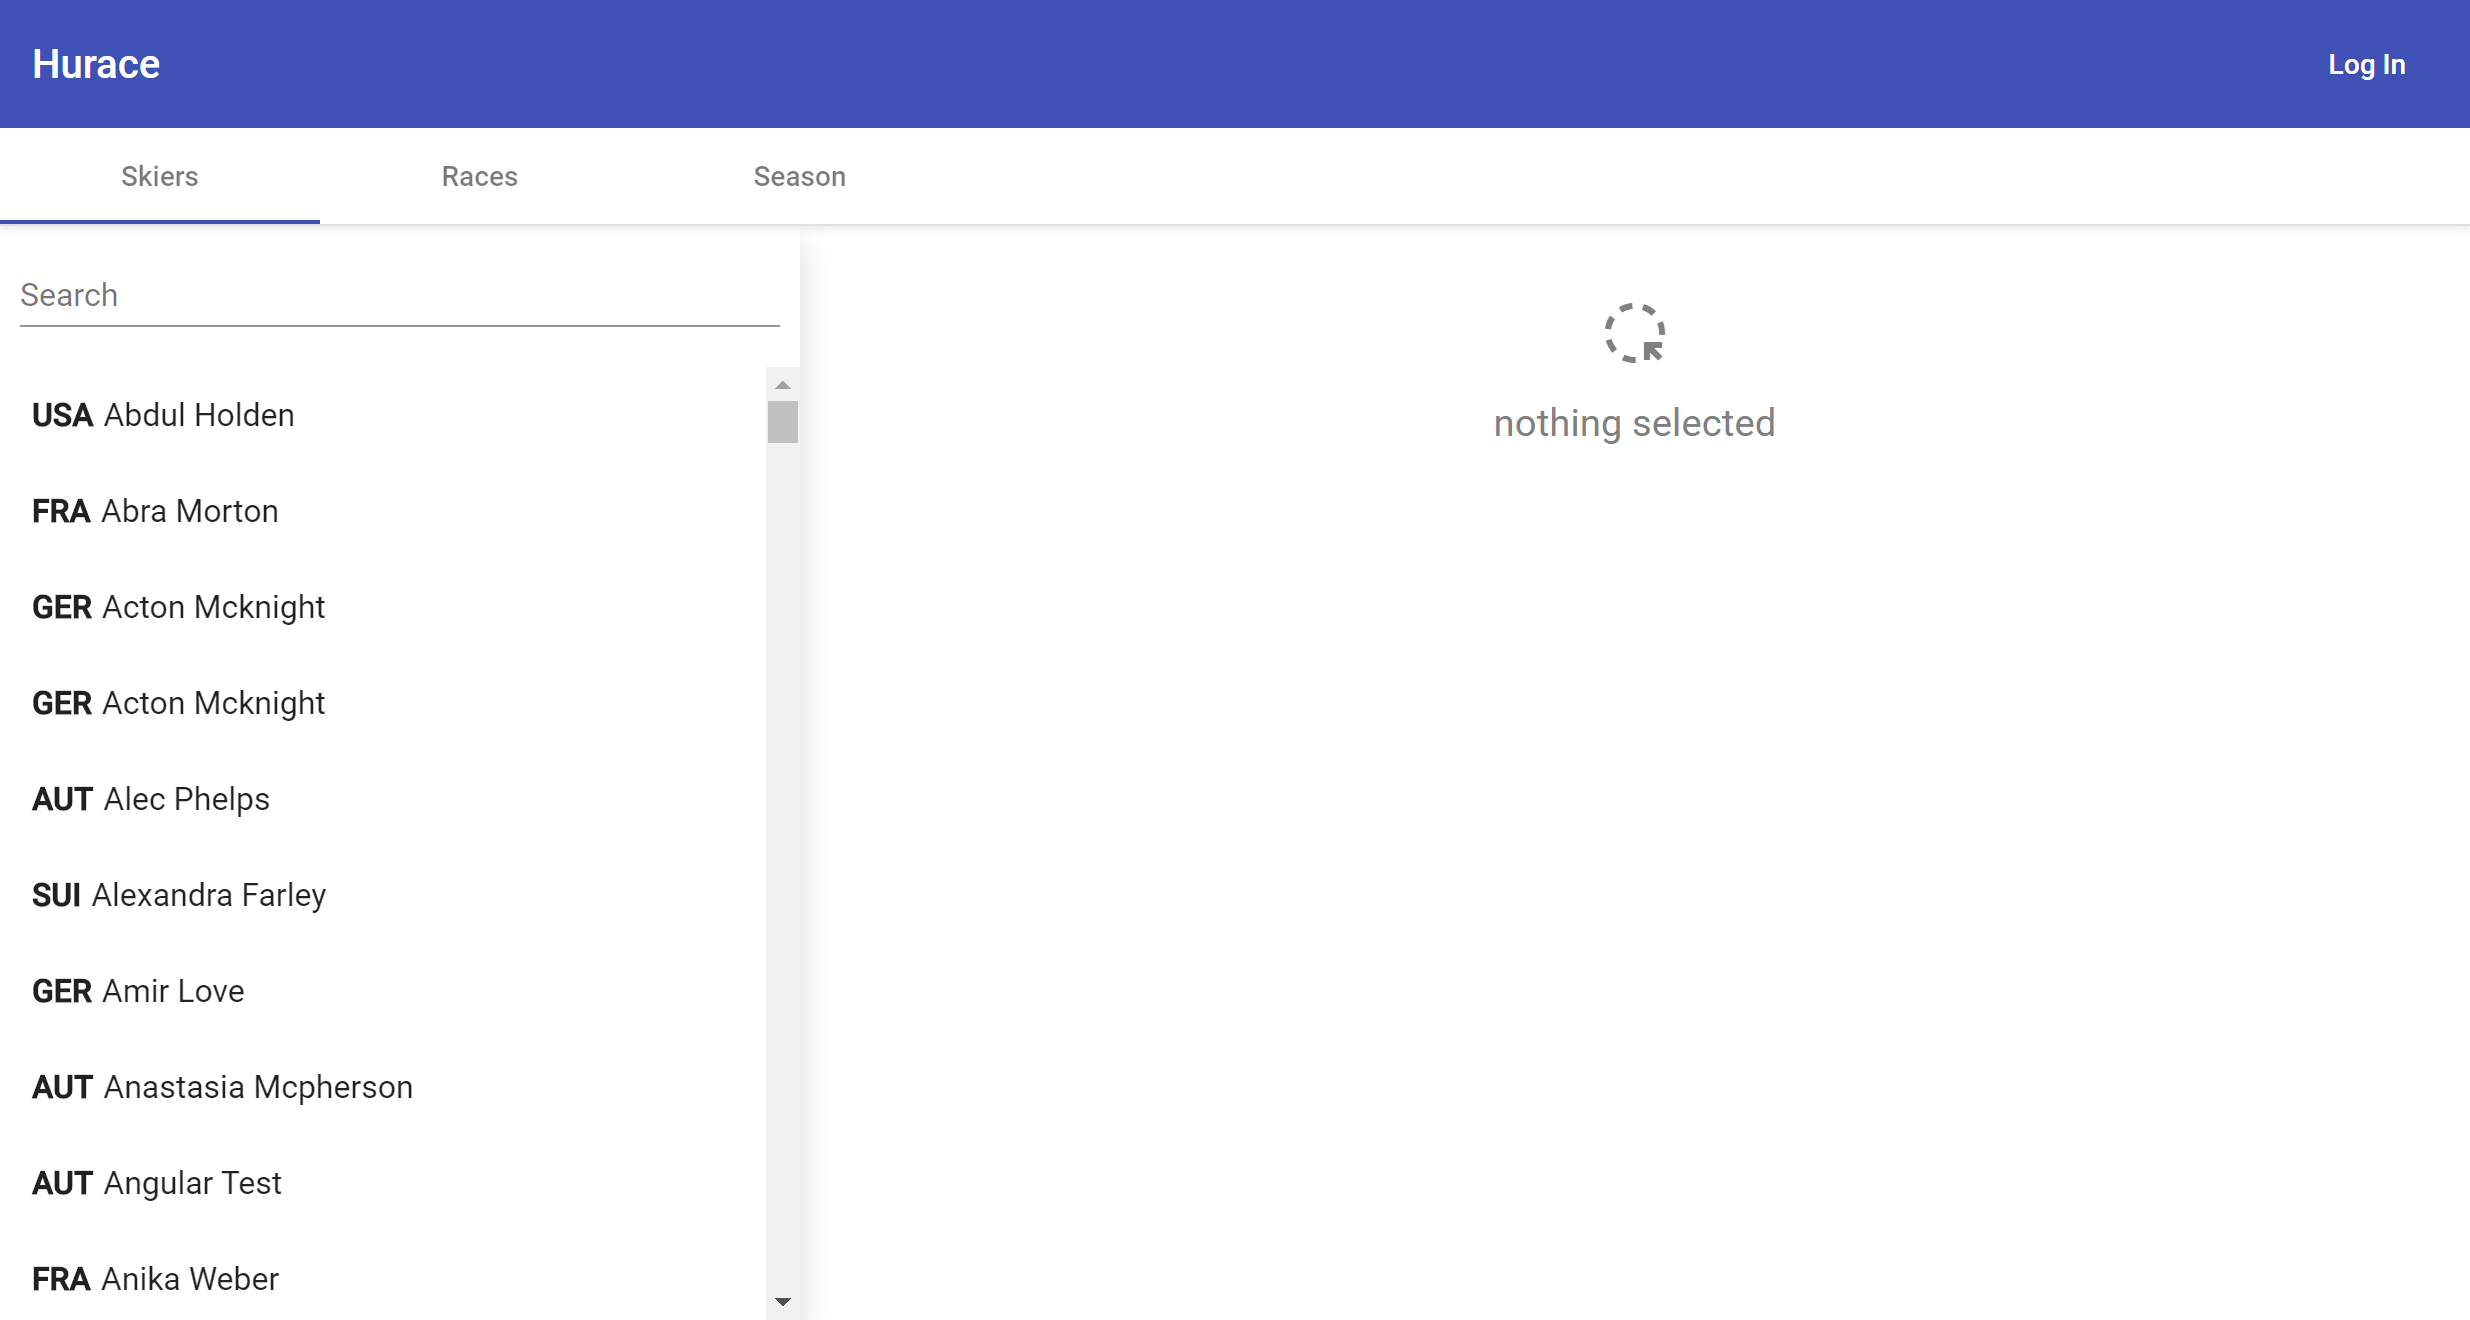
\includegraphics[width=0.9\linewidth]{images/skiers-list}
    \caption{Liste an SkirennläuferInnen}
\label{fig:skiers-list}
\end{figure}

Im Suchfeld kann nach Name oder Länderkürzel (\zB AUT, GER, ...) gefiltert werden (\cref{fig:skiers-search-success}).
\begin{figure}[H]
    \centering
    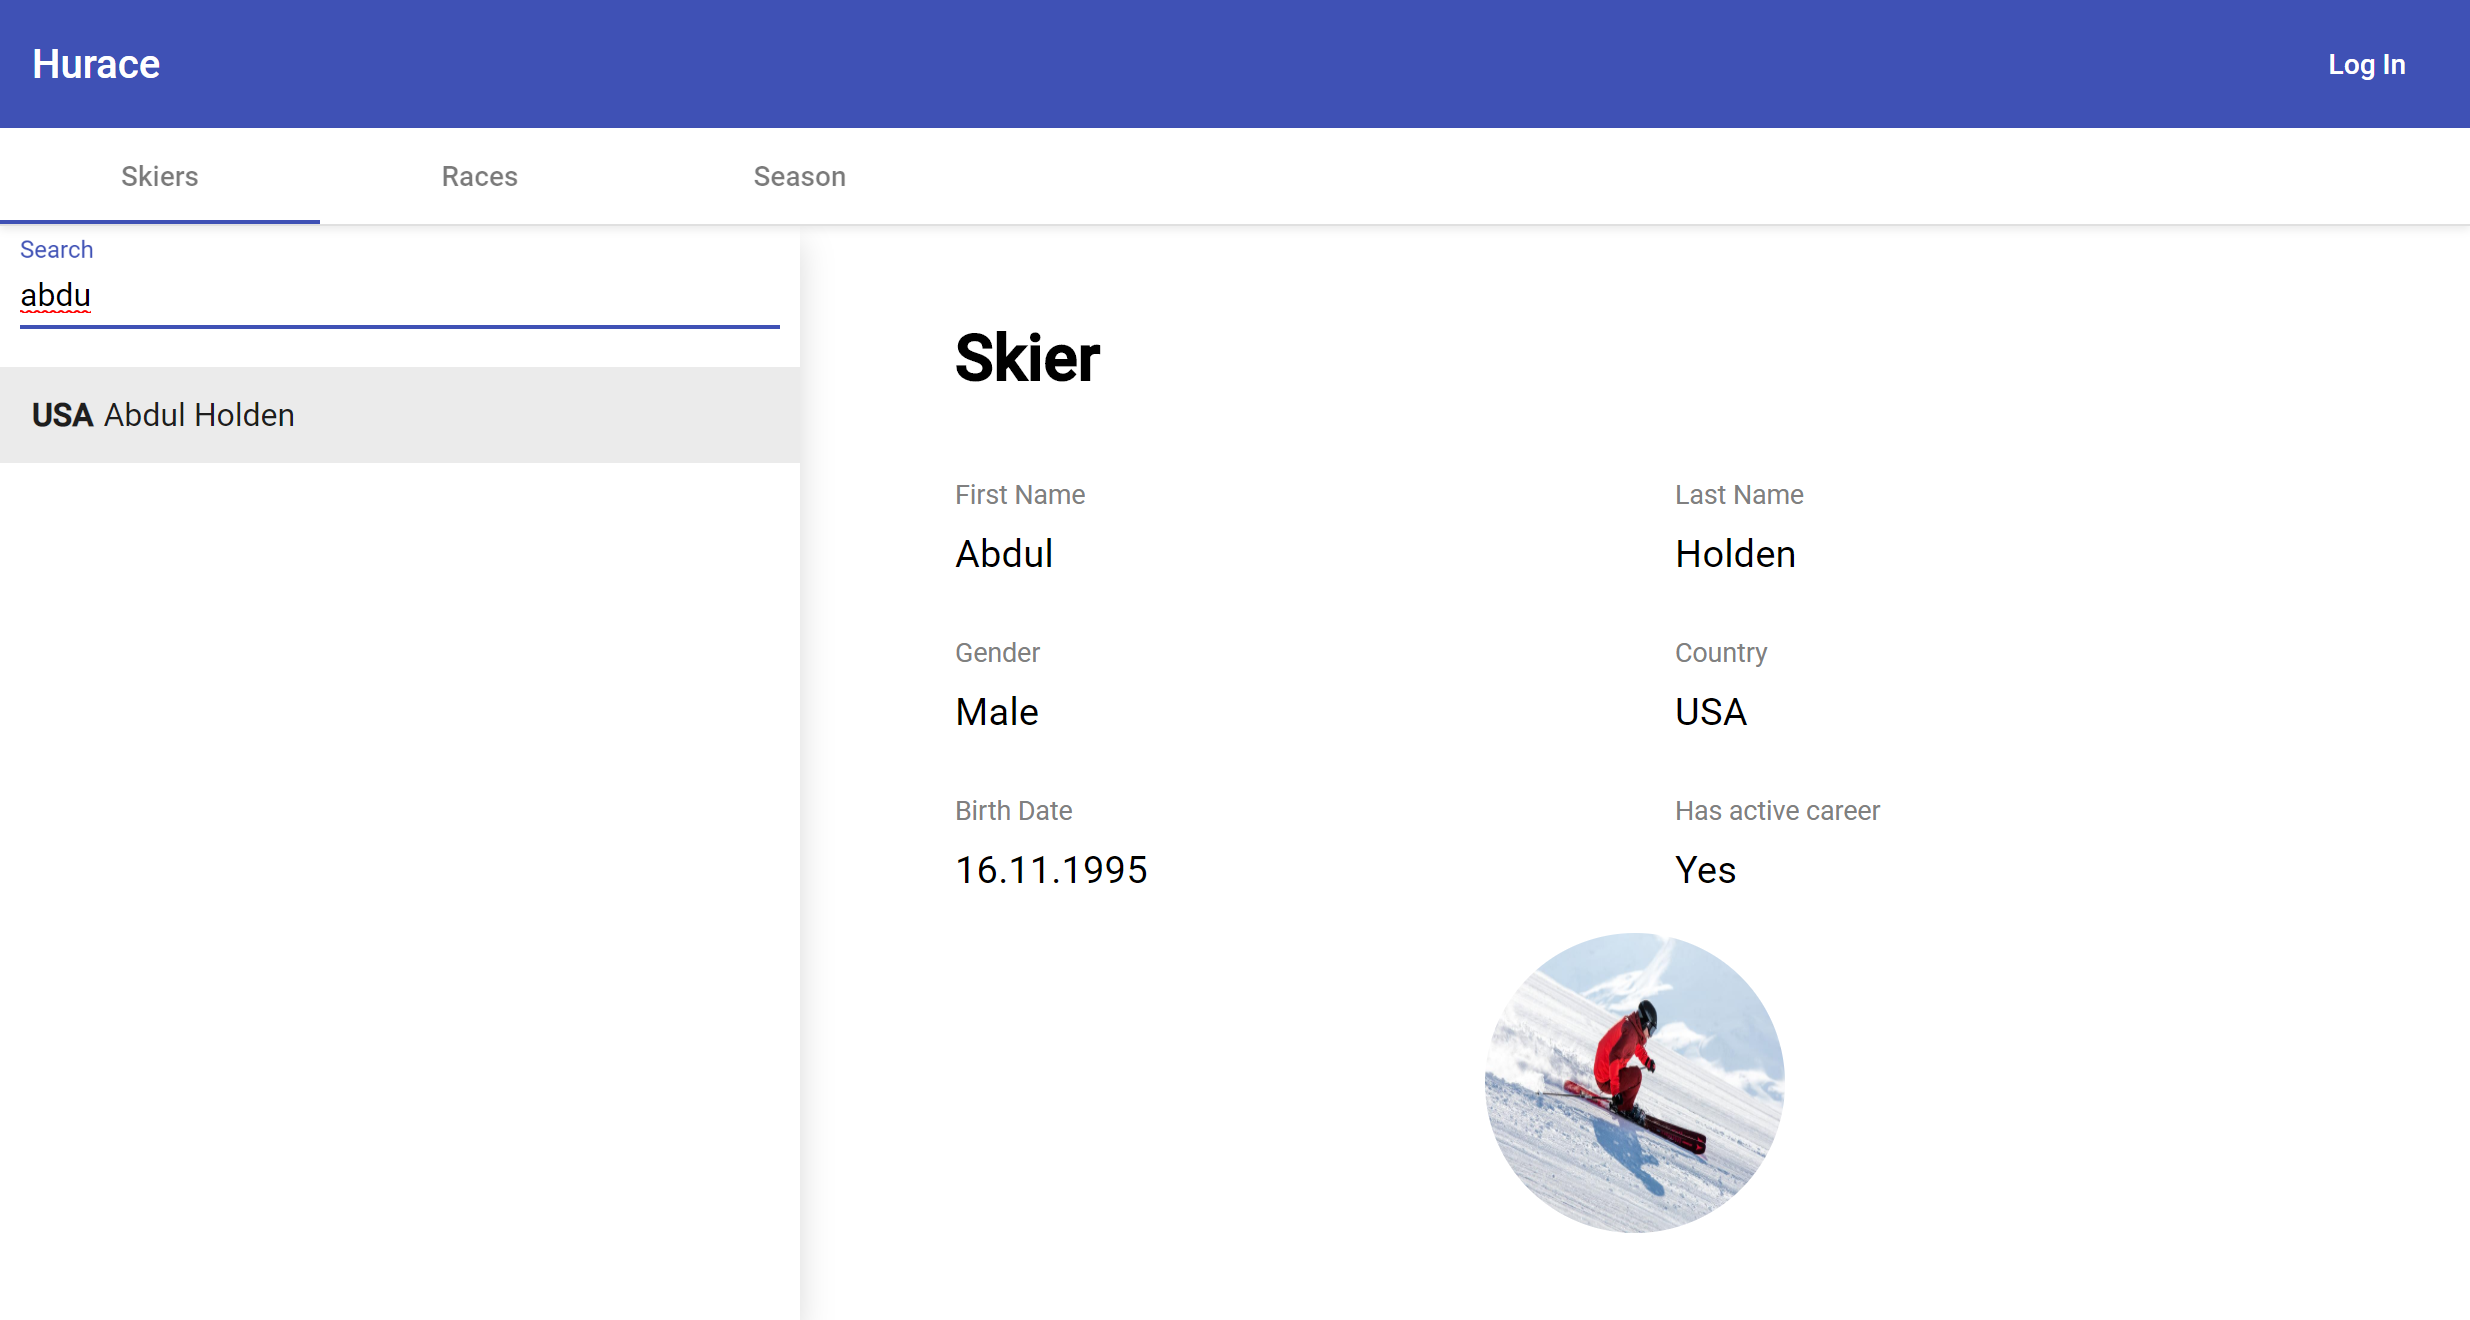
\includegraphics[width=0.9\linewidth]{images/skiers-search-success}
    \caption{Filtern der SkirennläuferInnen}
\label{fig:skiers-search-success}
\end{figure}

Wenn keine SkirennläuferIn gefunden wird wird eine entsprechende Meldung angezeigt (\cref{fig:skiers-search-error}).
\begin{figure}[H]
    \centering
    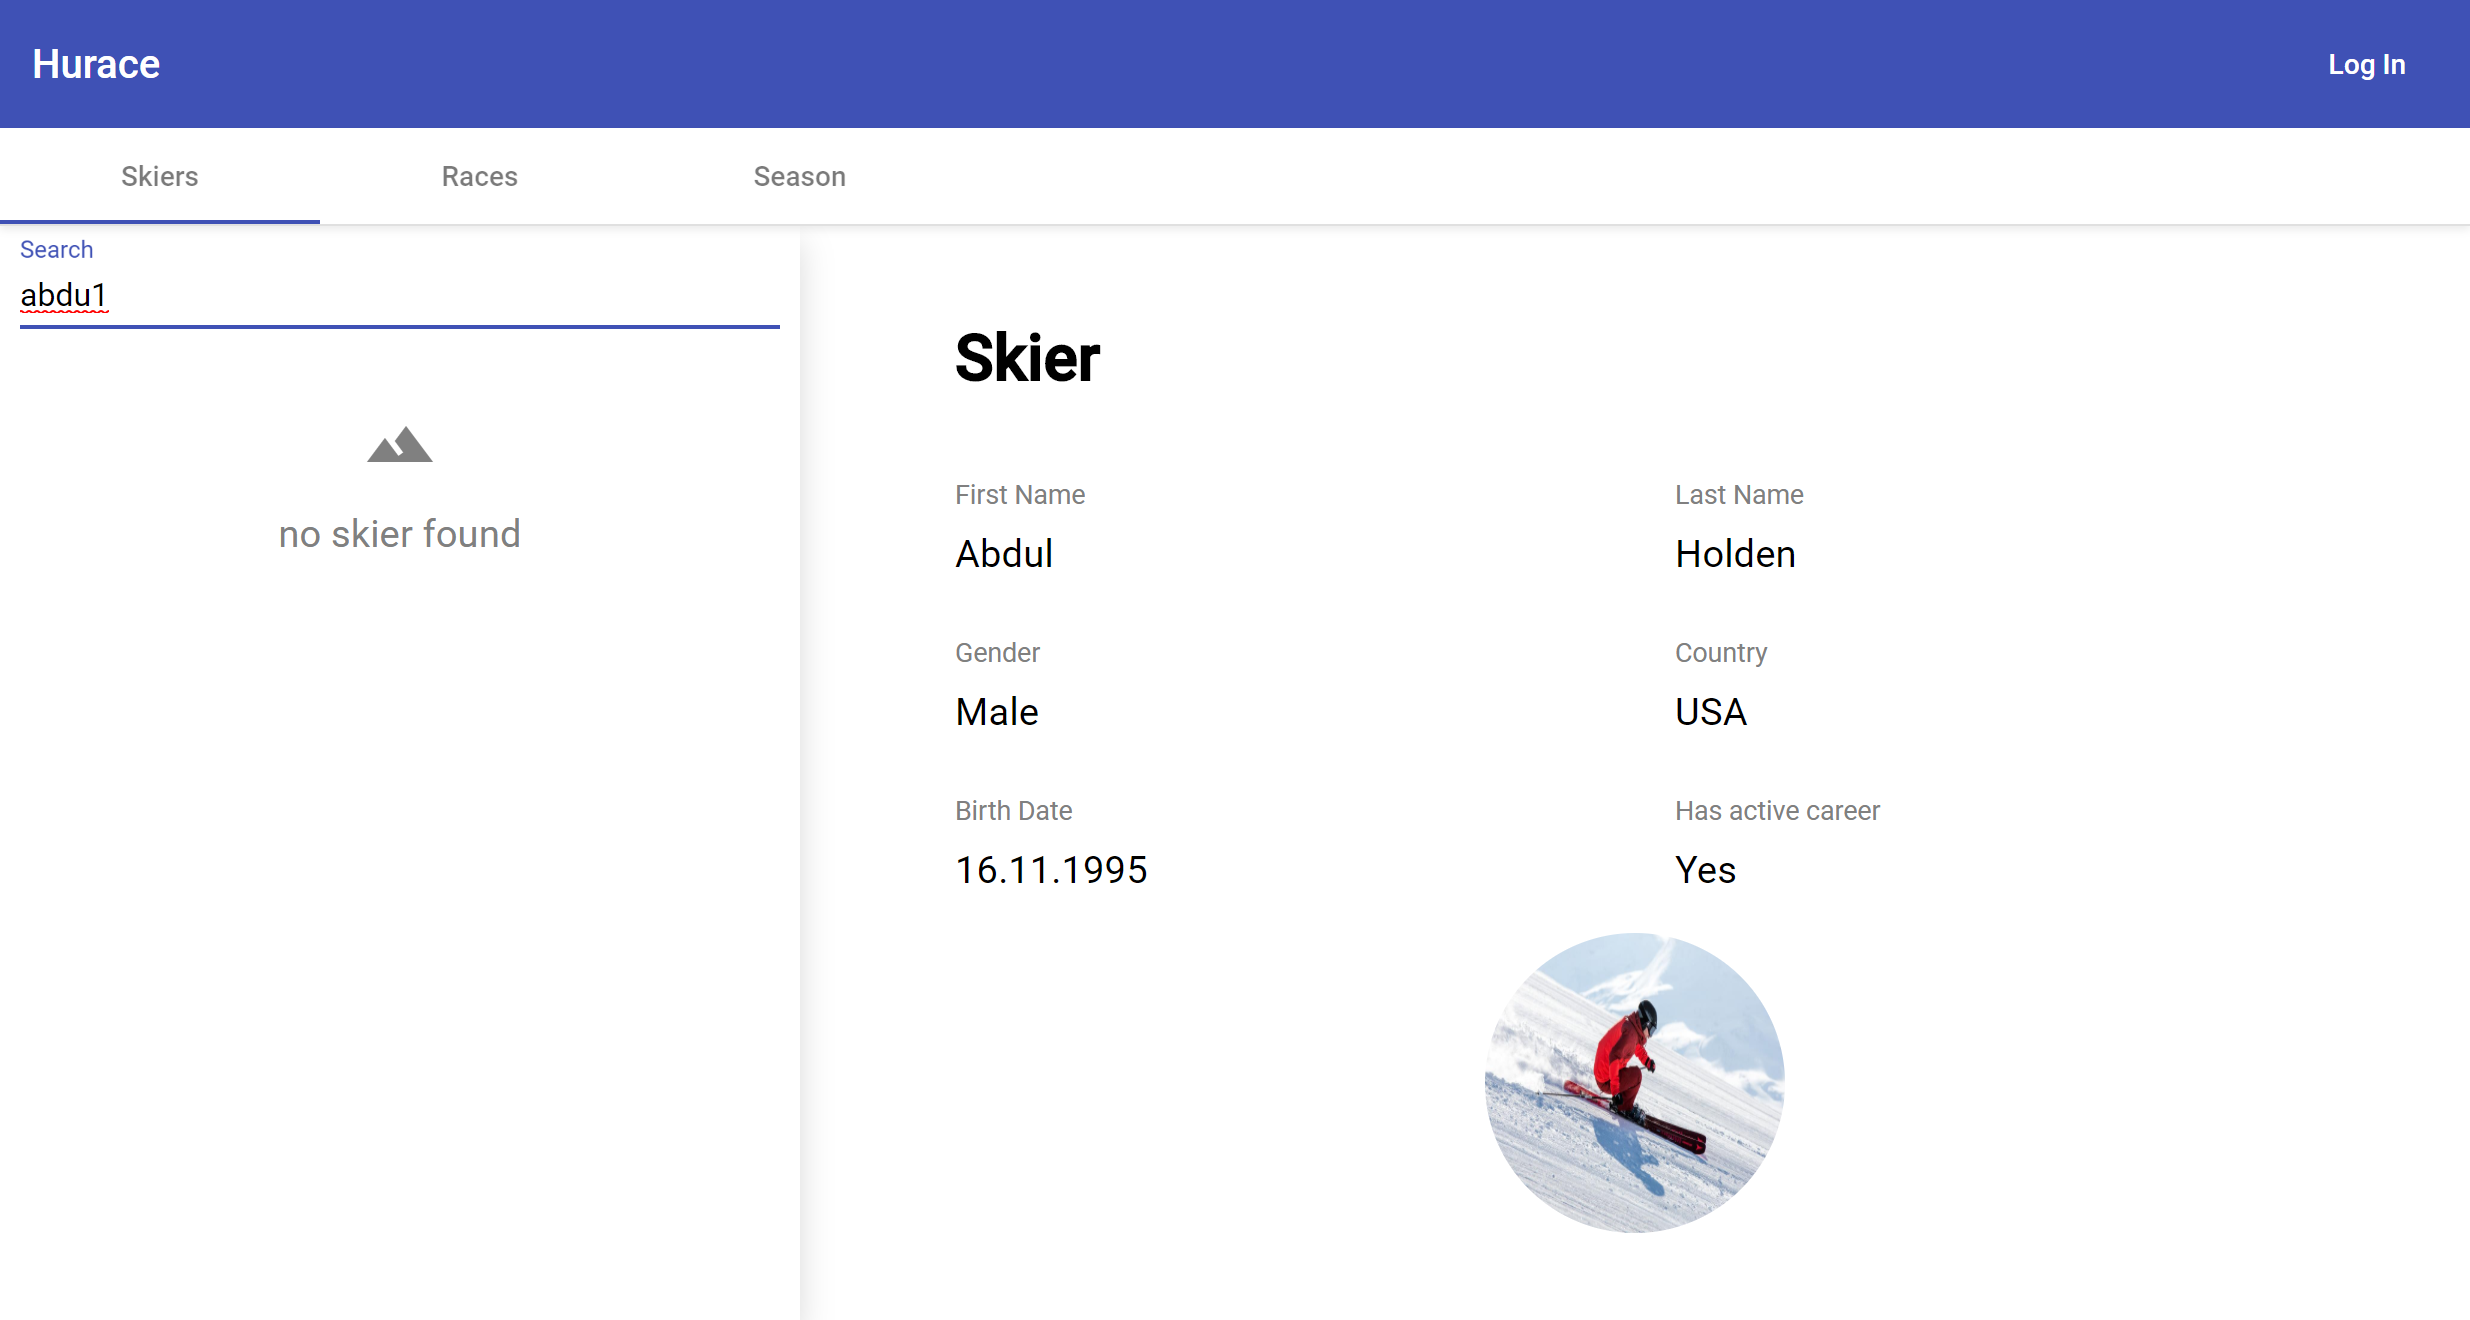
\includegraphics[width=0.9\linewidth]{images/skiers-search-error}
    \caption{Keine Ergebnisse beim Filtern der SkirennläuferInnen}
\label{fig:skiers-search-error}
\end{figure}

Beim Selektieren einer SkirennläuferIn werden weitere Daten angezeigt (\cref{fig:skiers-detail}).
Außerdem ändert sich die Browser-URL auf \emph{/skiers/:id}, sodass bei einem Neuladen die zuvor selektierte SkirennläuferIn angezeigt wird.
\begin{figure}[H]
    \centering
    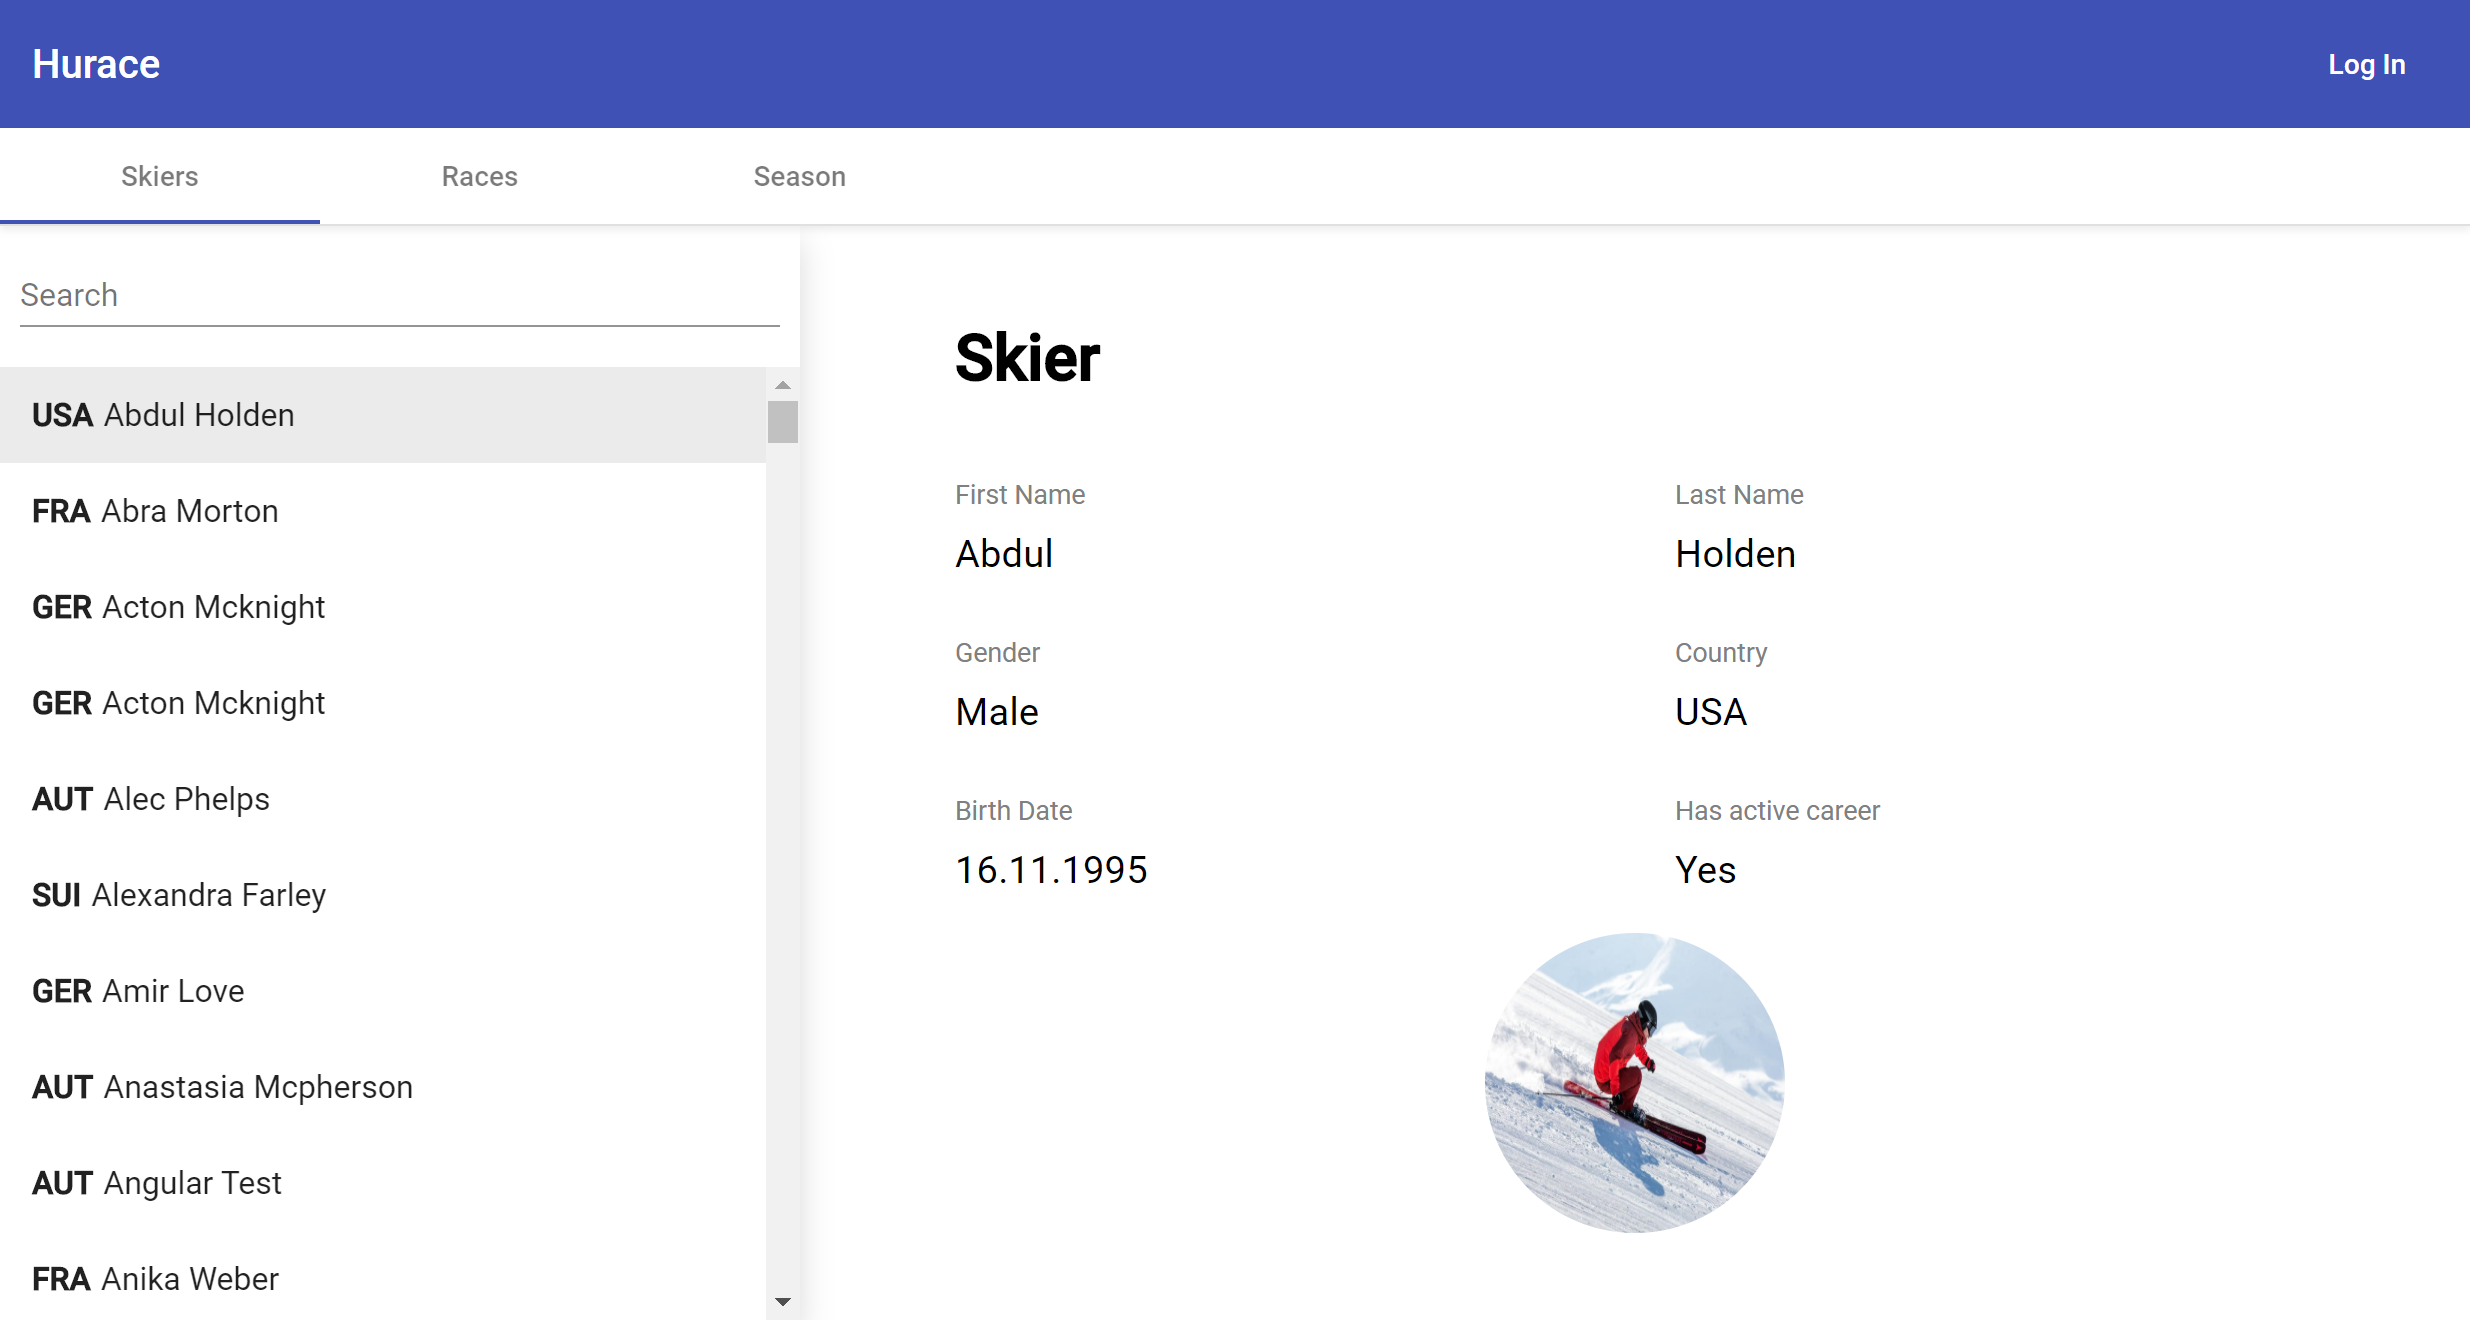
\includegraphics[width=0.9\linewidth]{images/skiers-detail}
    \caption{Detailansicht eines Skirennläufer}
\label{fig:skiers-detail}
\end{figure}

Falls der Anwender angemeldet ist können auch die SkirennläuferInnen bearbeitet oder gelöscht werden (\cref{fig:skiers-form}).
Außerdem können neue SkirennläuferInnen über die \emph{New}-Schaltfläche hinzugefügt werden.
\begin{figure}[H]
    \centering
    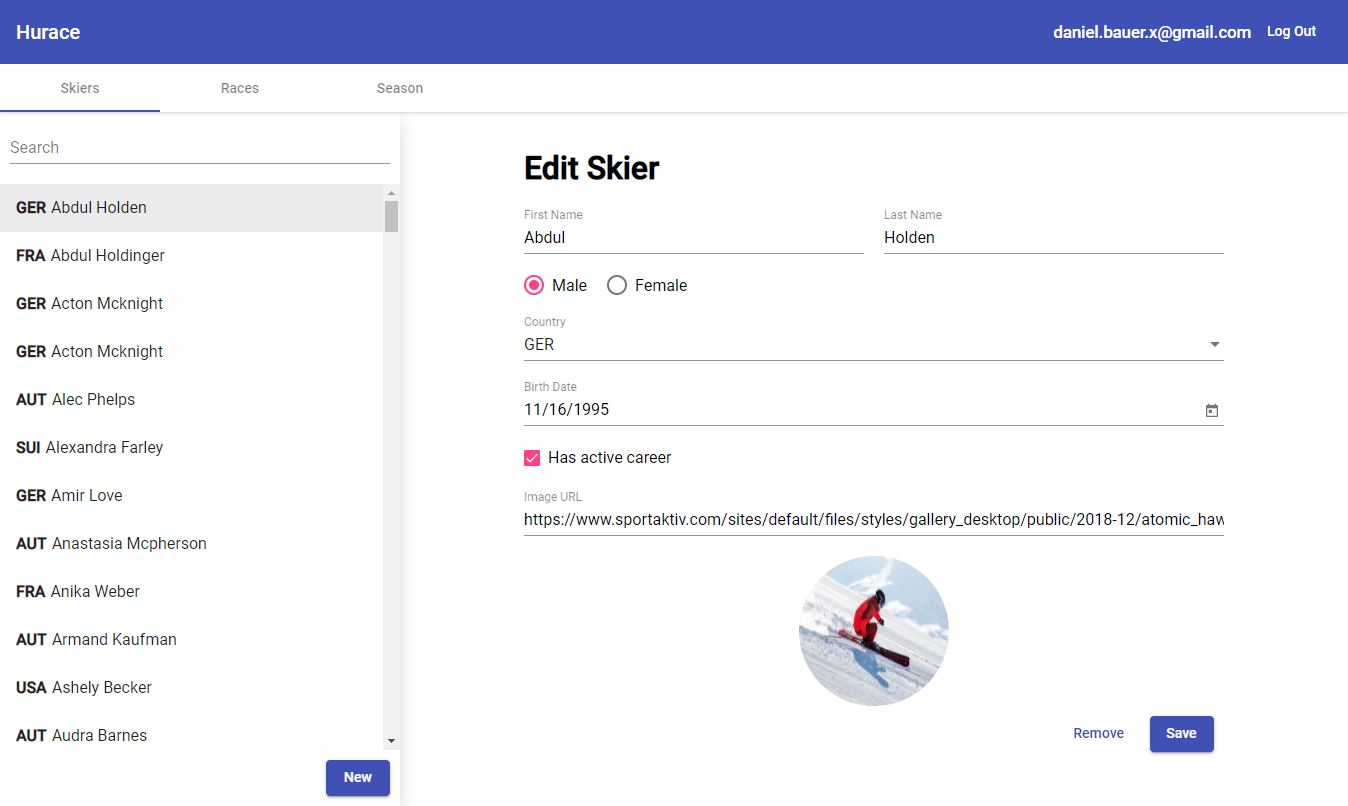
\includegraphics[width=0.9\linewidth]{images/skiers-form}
    \caption{Stammdatenverwaltung eines Skirennläufers}
\label{fig:skiers-form}
\end{figure}

\section{Races}
Die \emph{Races}-Seite zeigt eine Liste von allen Rennen nach Datum sortiert an (\cref{fig:races-list}).
\begin{figure}[H]
    \centering
    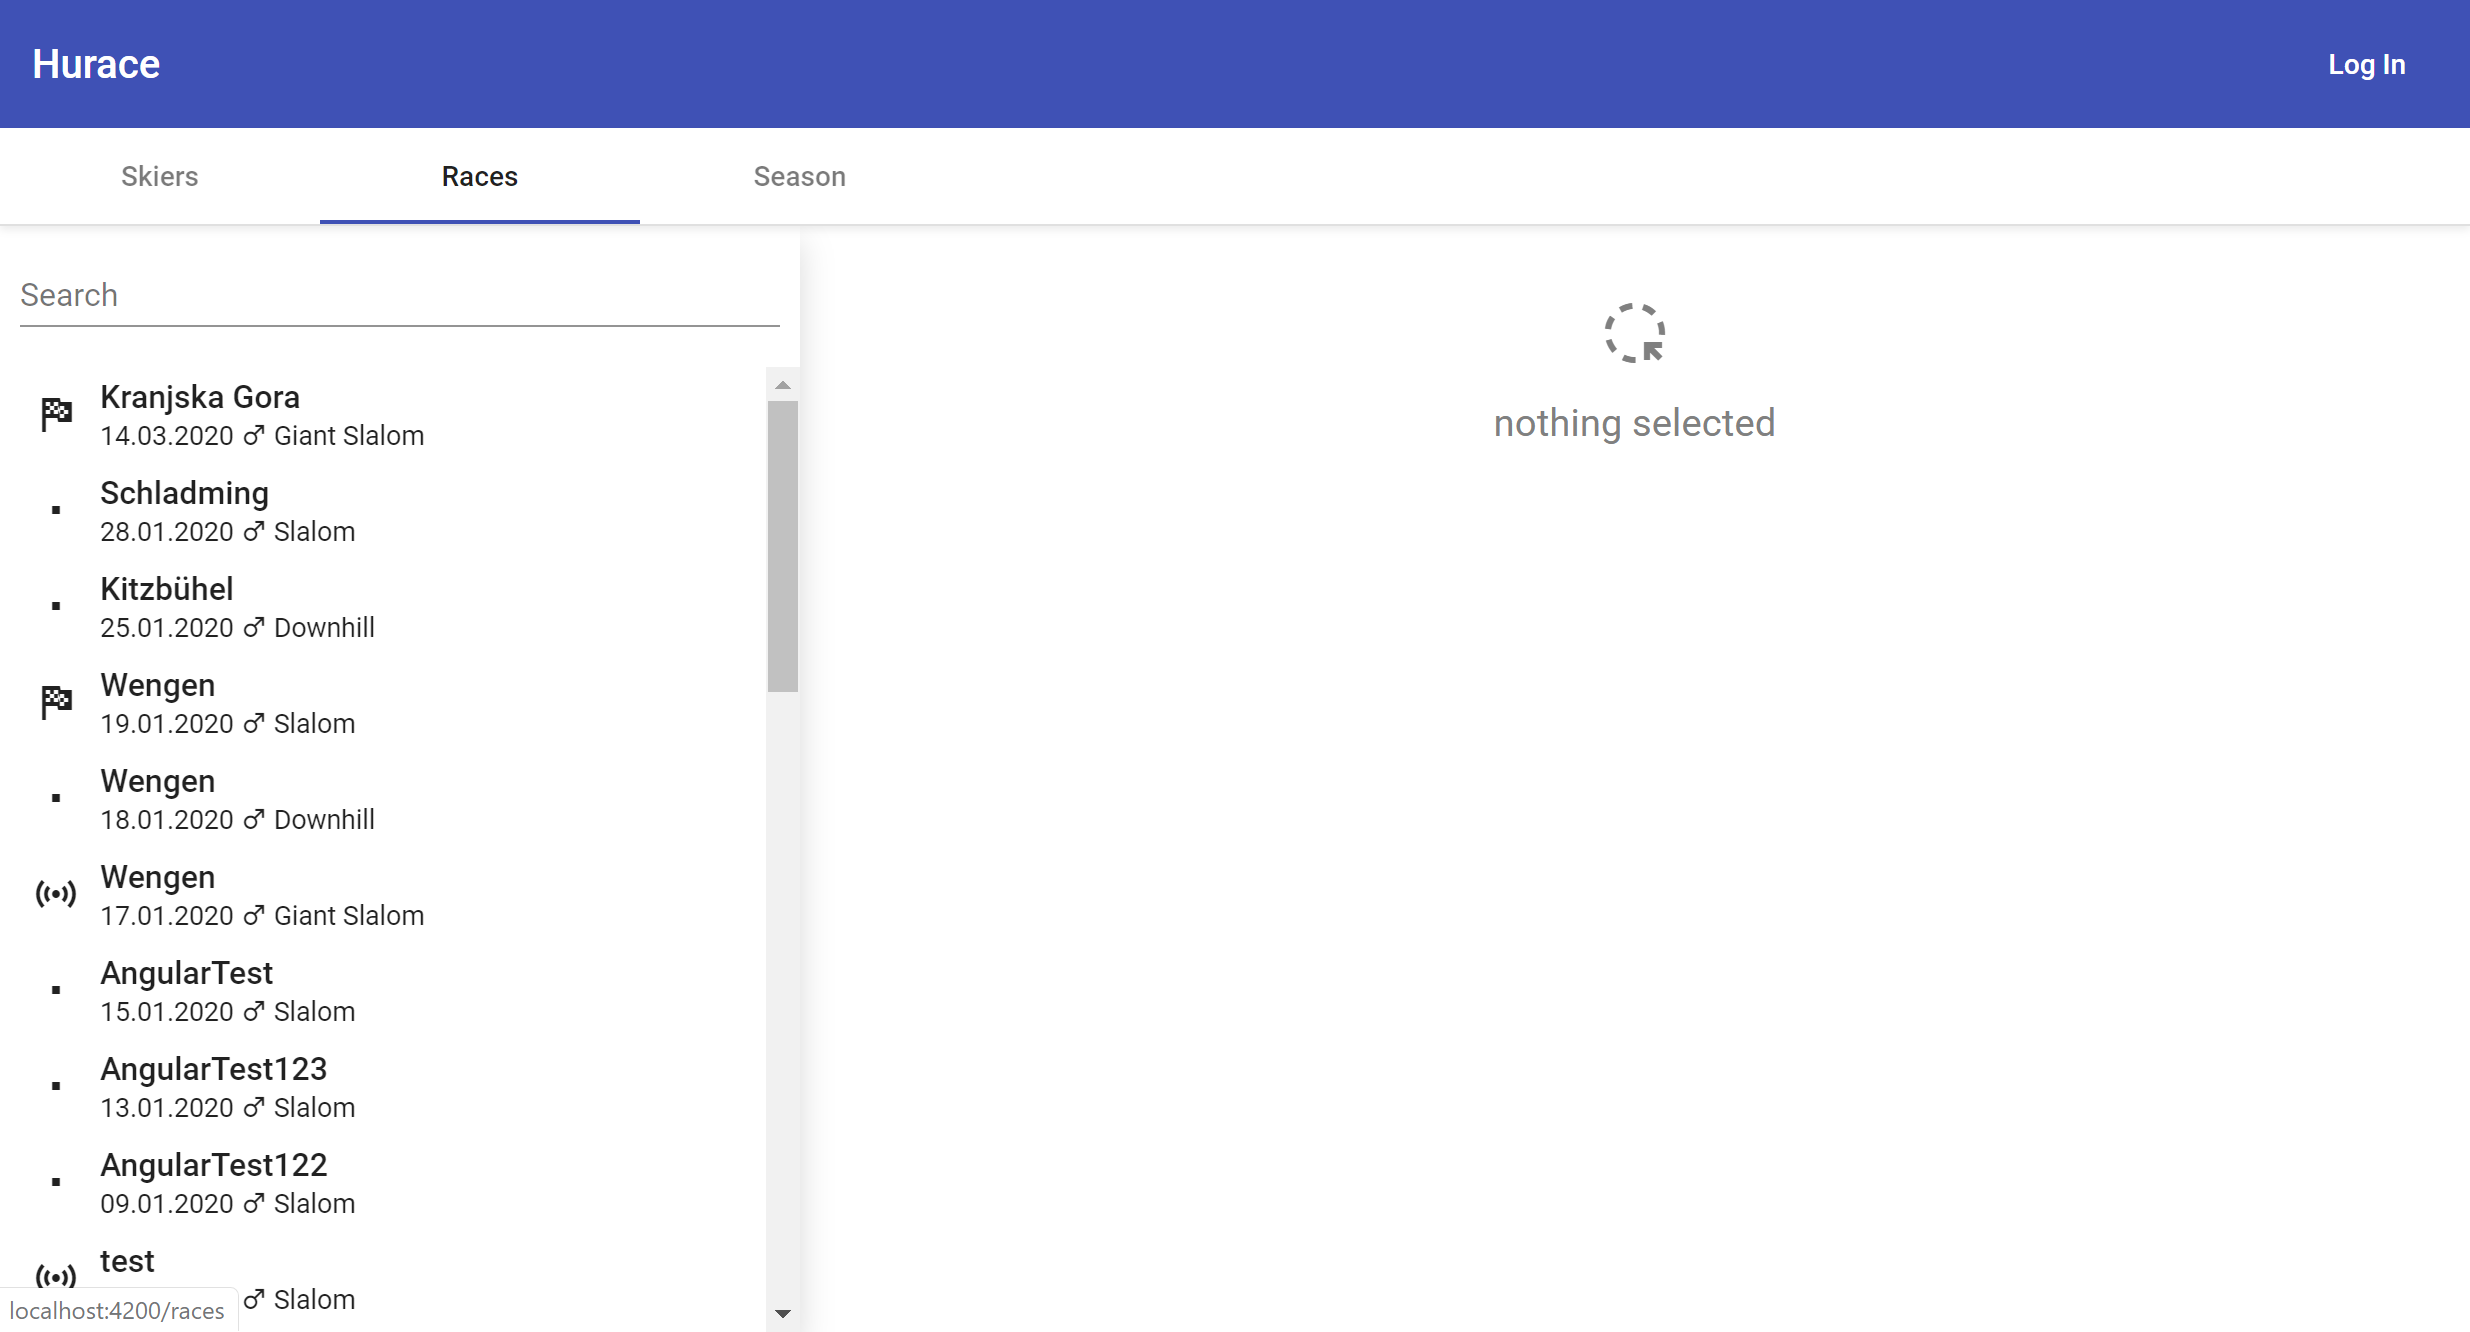
\includegraphics[width=0.9\linewidth]{images/races-list}
    \caption{Liste an Rennen}
\label{fig:races-list}
\end{figure}

Im Suchfeld kann nach Name gefiltert werden (\cref{fig:races-search-success}).
\begin{figure}[H]
    \centering
    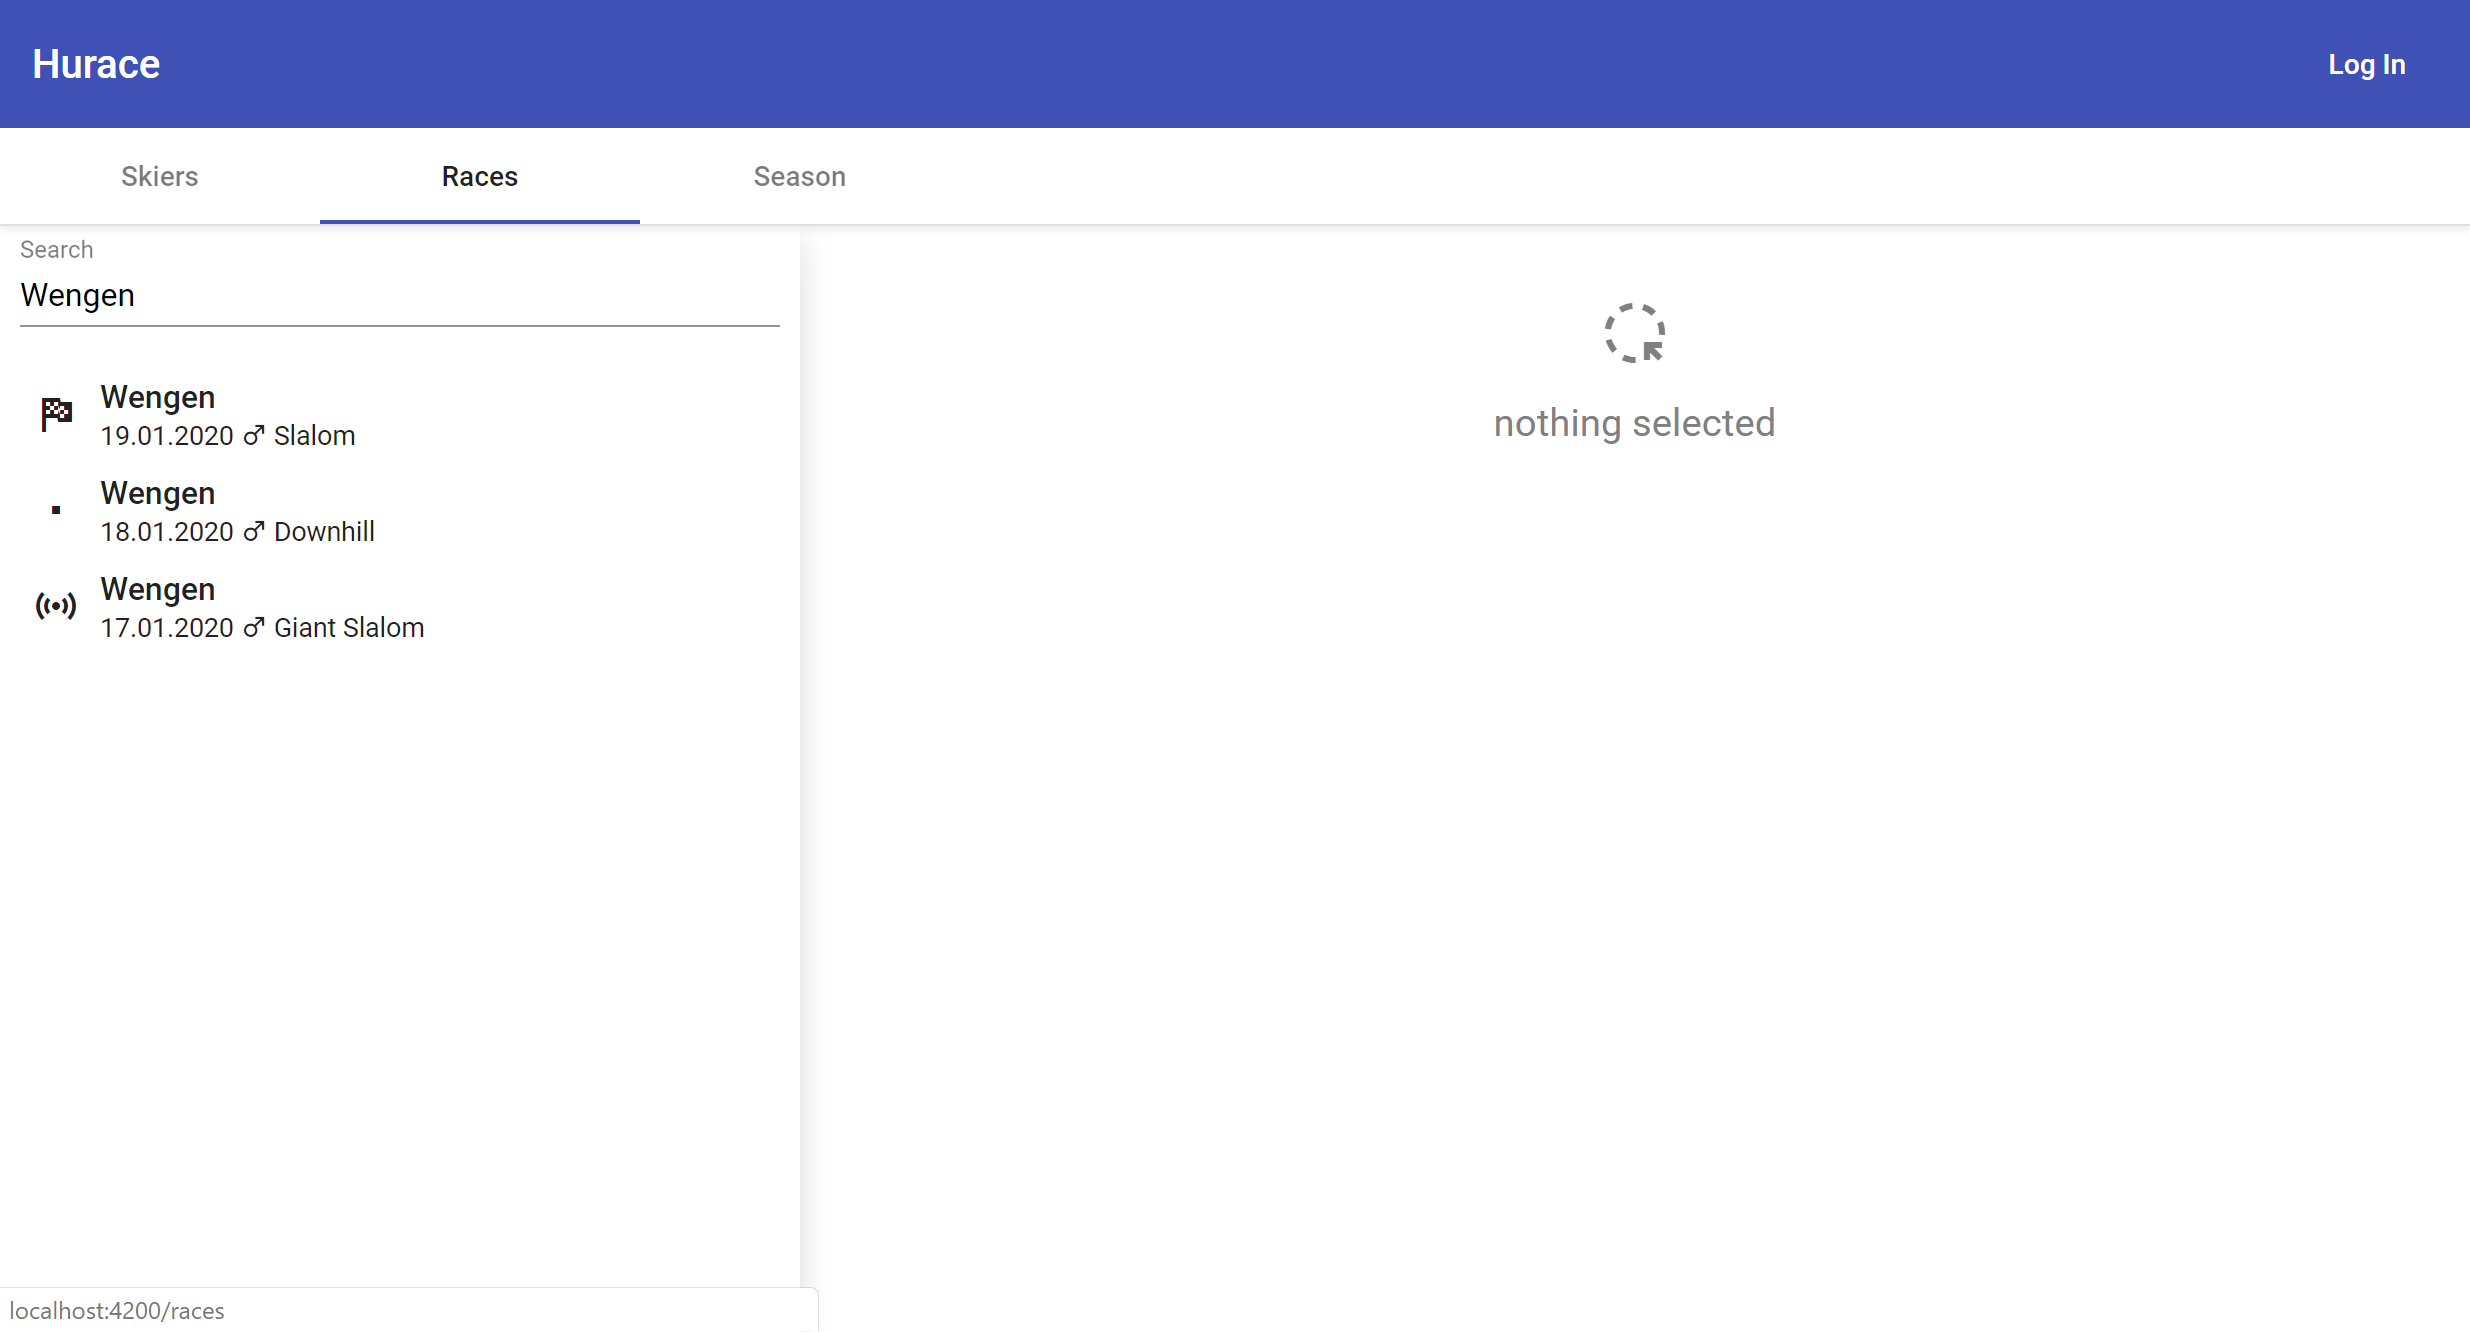
\includegraphics[width=0.9\linewidth]{images/races-search-success}
    \caption{Filtern der Rennen}
\label{fig:races-search-success}
\end{figure}

Wenn kein Rennen gefunden wird, wird eine entsprechende Meldung angezeigt (\cref{fig:races-search-error}).
\begin{figure}[H]
    \centering
    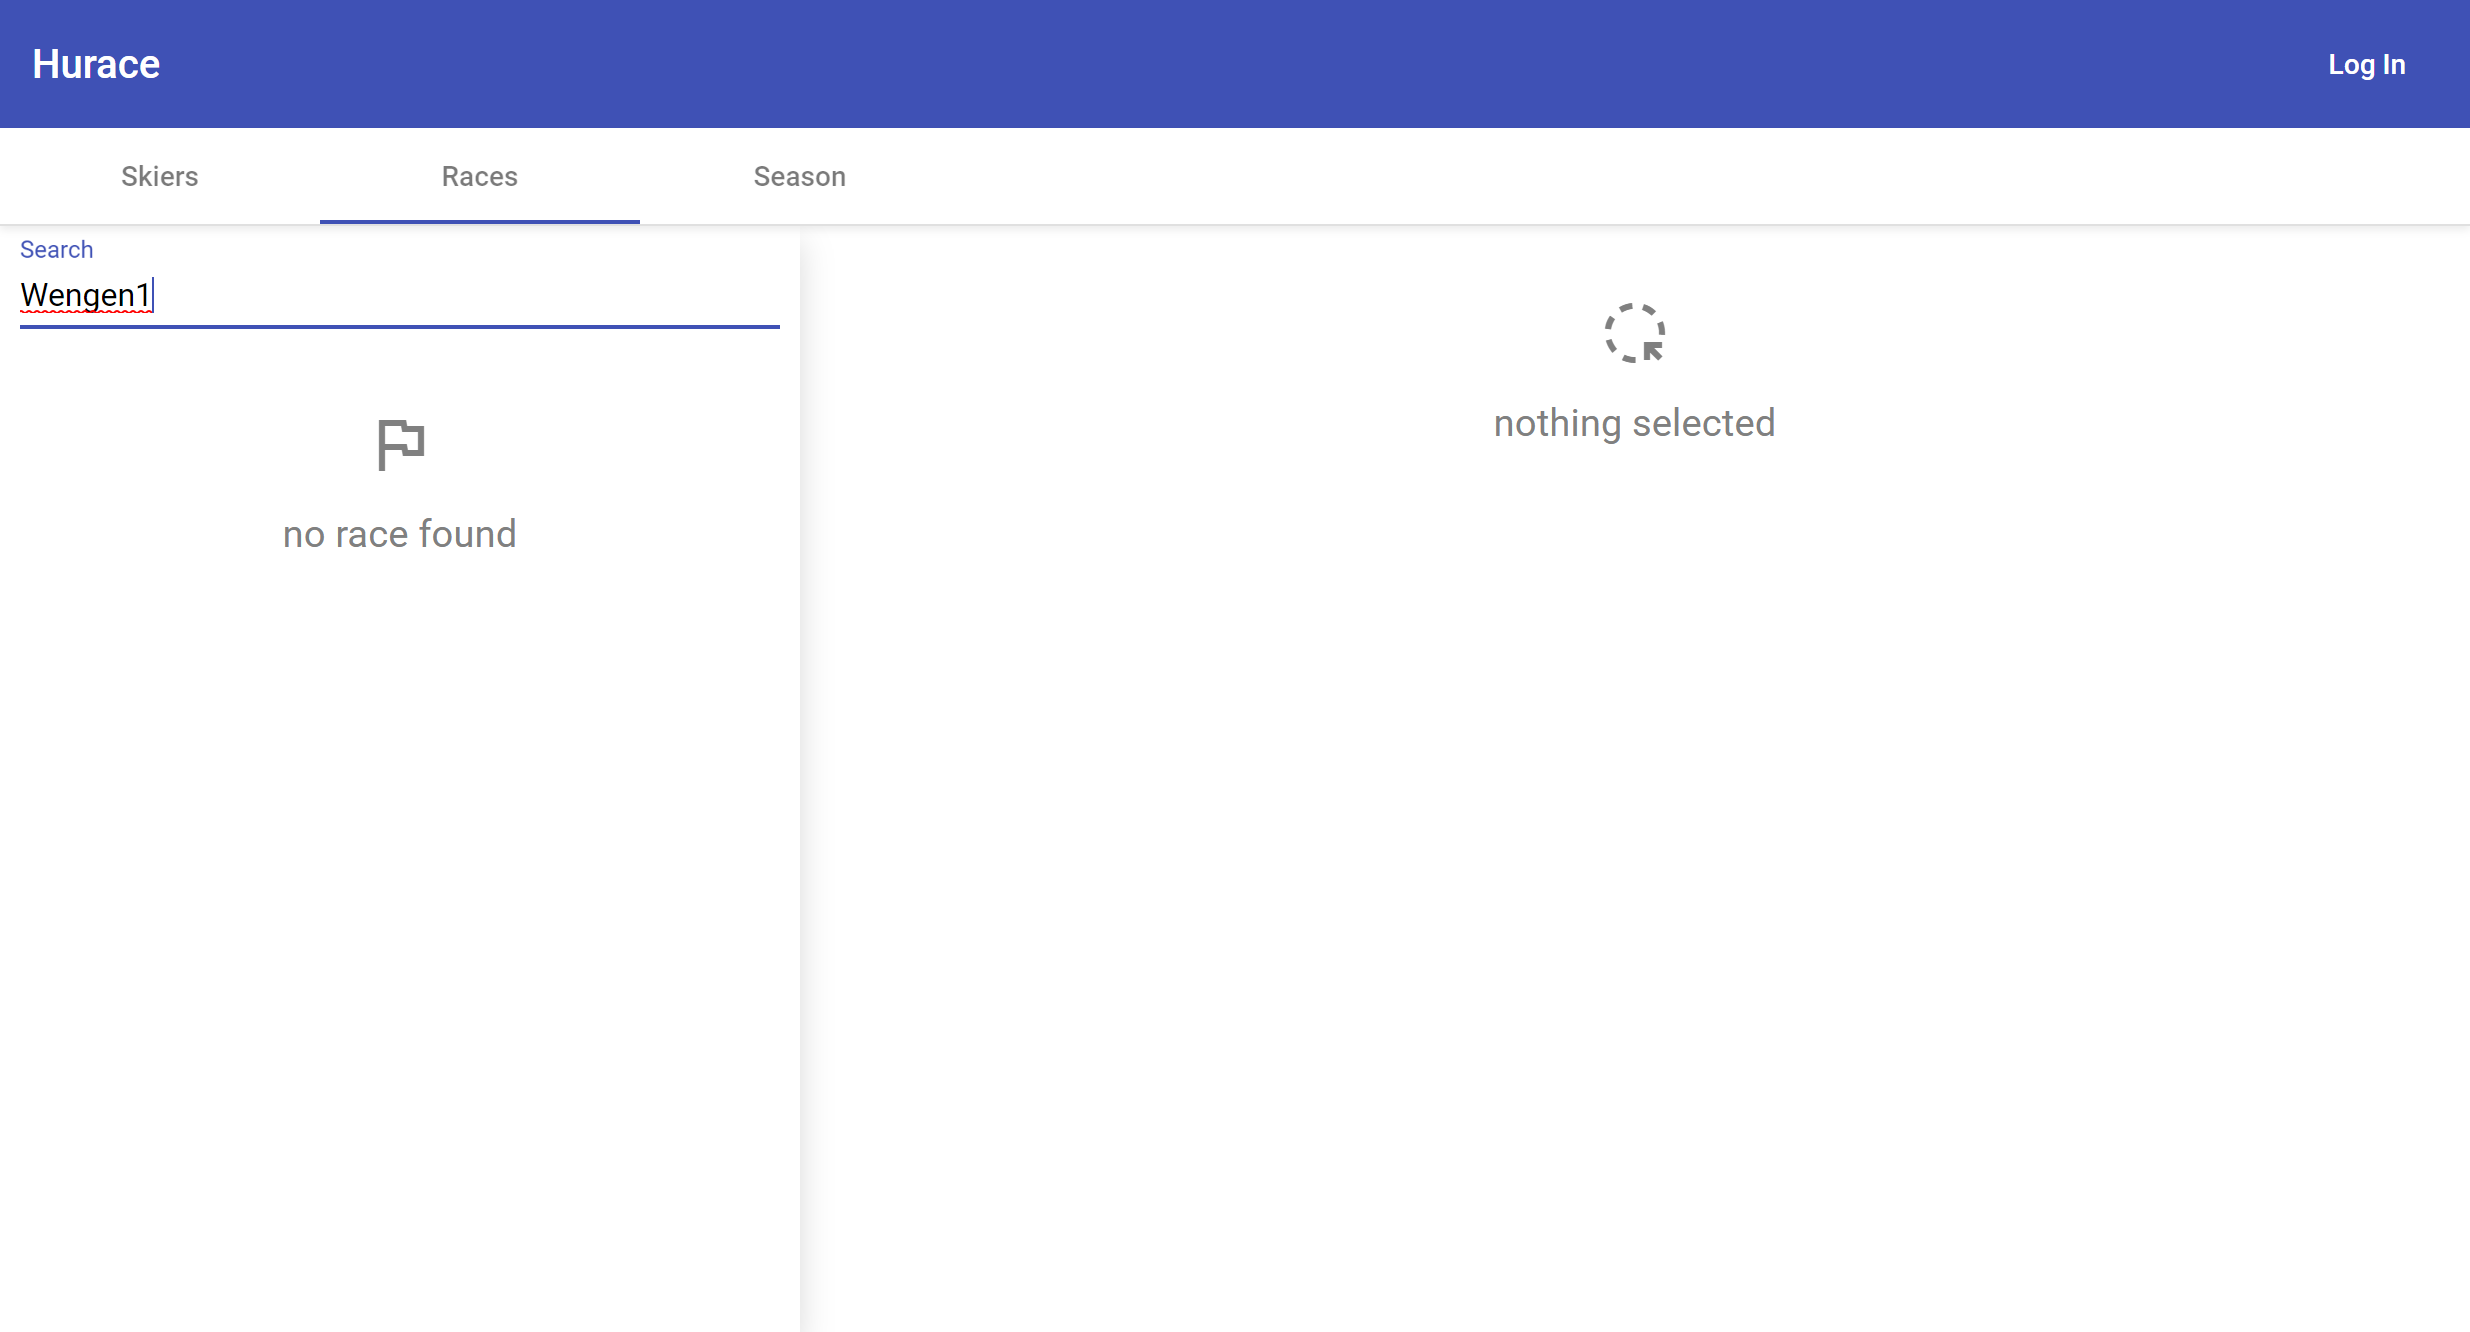
\includegraphics[width=0.9\linewidth]{images/races-search-error}
    \caption{Keine Ergebnisse beim Filtern der Rennen}
\label{fig:races-search-error}
\end{figure}

Beim Selektieren eines Rennens werden weitere Detaildaten angezeigt (\cref{fig:races-detail}).
Außerdem ändert sich die Browser-URL auf \emph{/races/:id}, sodass bei einem Neuladen das zuvor selektierte Rennen angezeigt wird.
Je nach Rennstatus werden unterschiedliche Detaildaten angezeigt:

\begin{description}
    \item[Abgeschlossenes Rennen:] Es werden die Endergebnisse der Durchgänge angezeigt. Bei Rennen mit zwei Durchgänge kann auch der Zwischenstand des ersten Durchgangs angsehen werden (\cref{fig:races-detail}).
    \item[Laufendes Rennen:] Bei einem laufendem Rennen wird zusätzlich zu den Ergebnissen die aktuelle SkirennläuferIn und deren Zwischenzeiten angezeigt (\cref{fig:races-live}).
    \item[Nicht gestartetes Rennen:] Der Benutzer wird mit der Meldung vertröstet, dass das Rennen erst zu einem späteren Zeitpunkt stattfindet (\cref{fig:races-not-started}).
\end{description}

\begin{figure}[H]
    \centering
    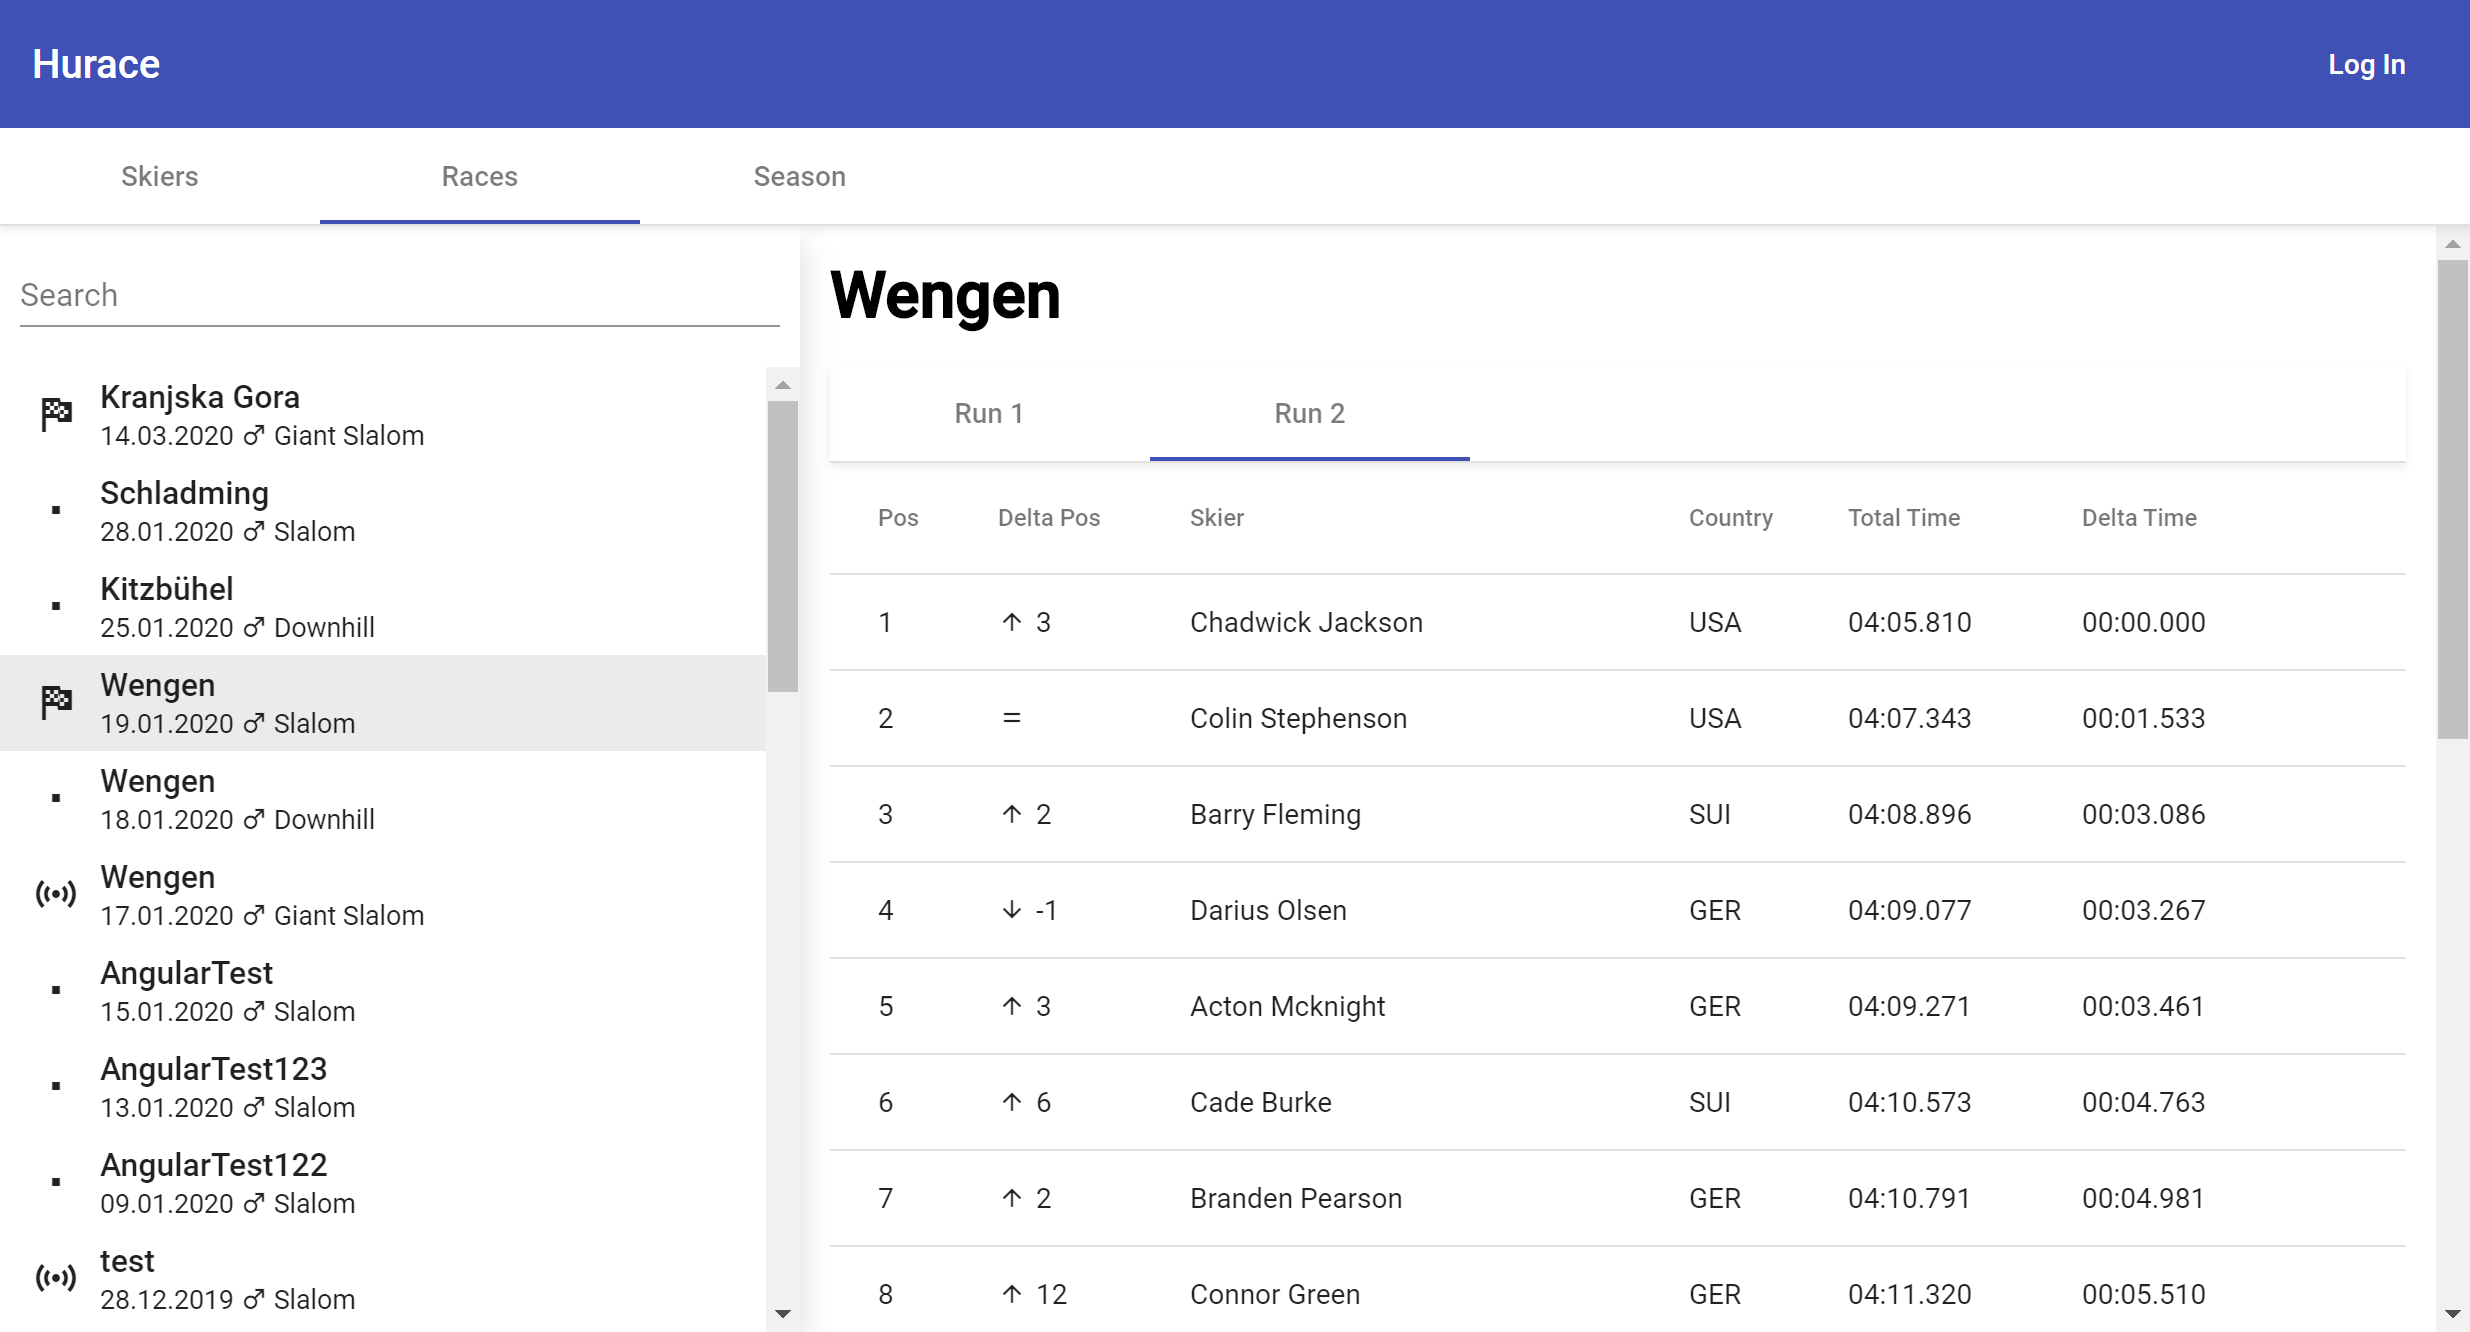
\includegraphics[width=0.9\linewidth]{images/races-detail}
    \caption{Detailansicht eines abgeschlossenen Rennens}
\label{fig:races-detail}
\end{figure}

\begin{figure}[H]
    \centering
    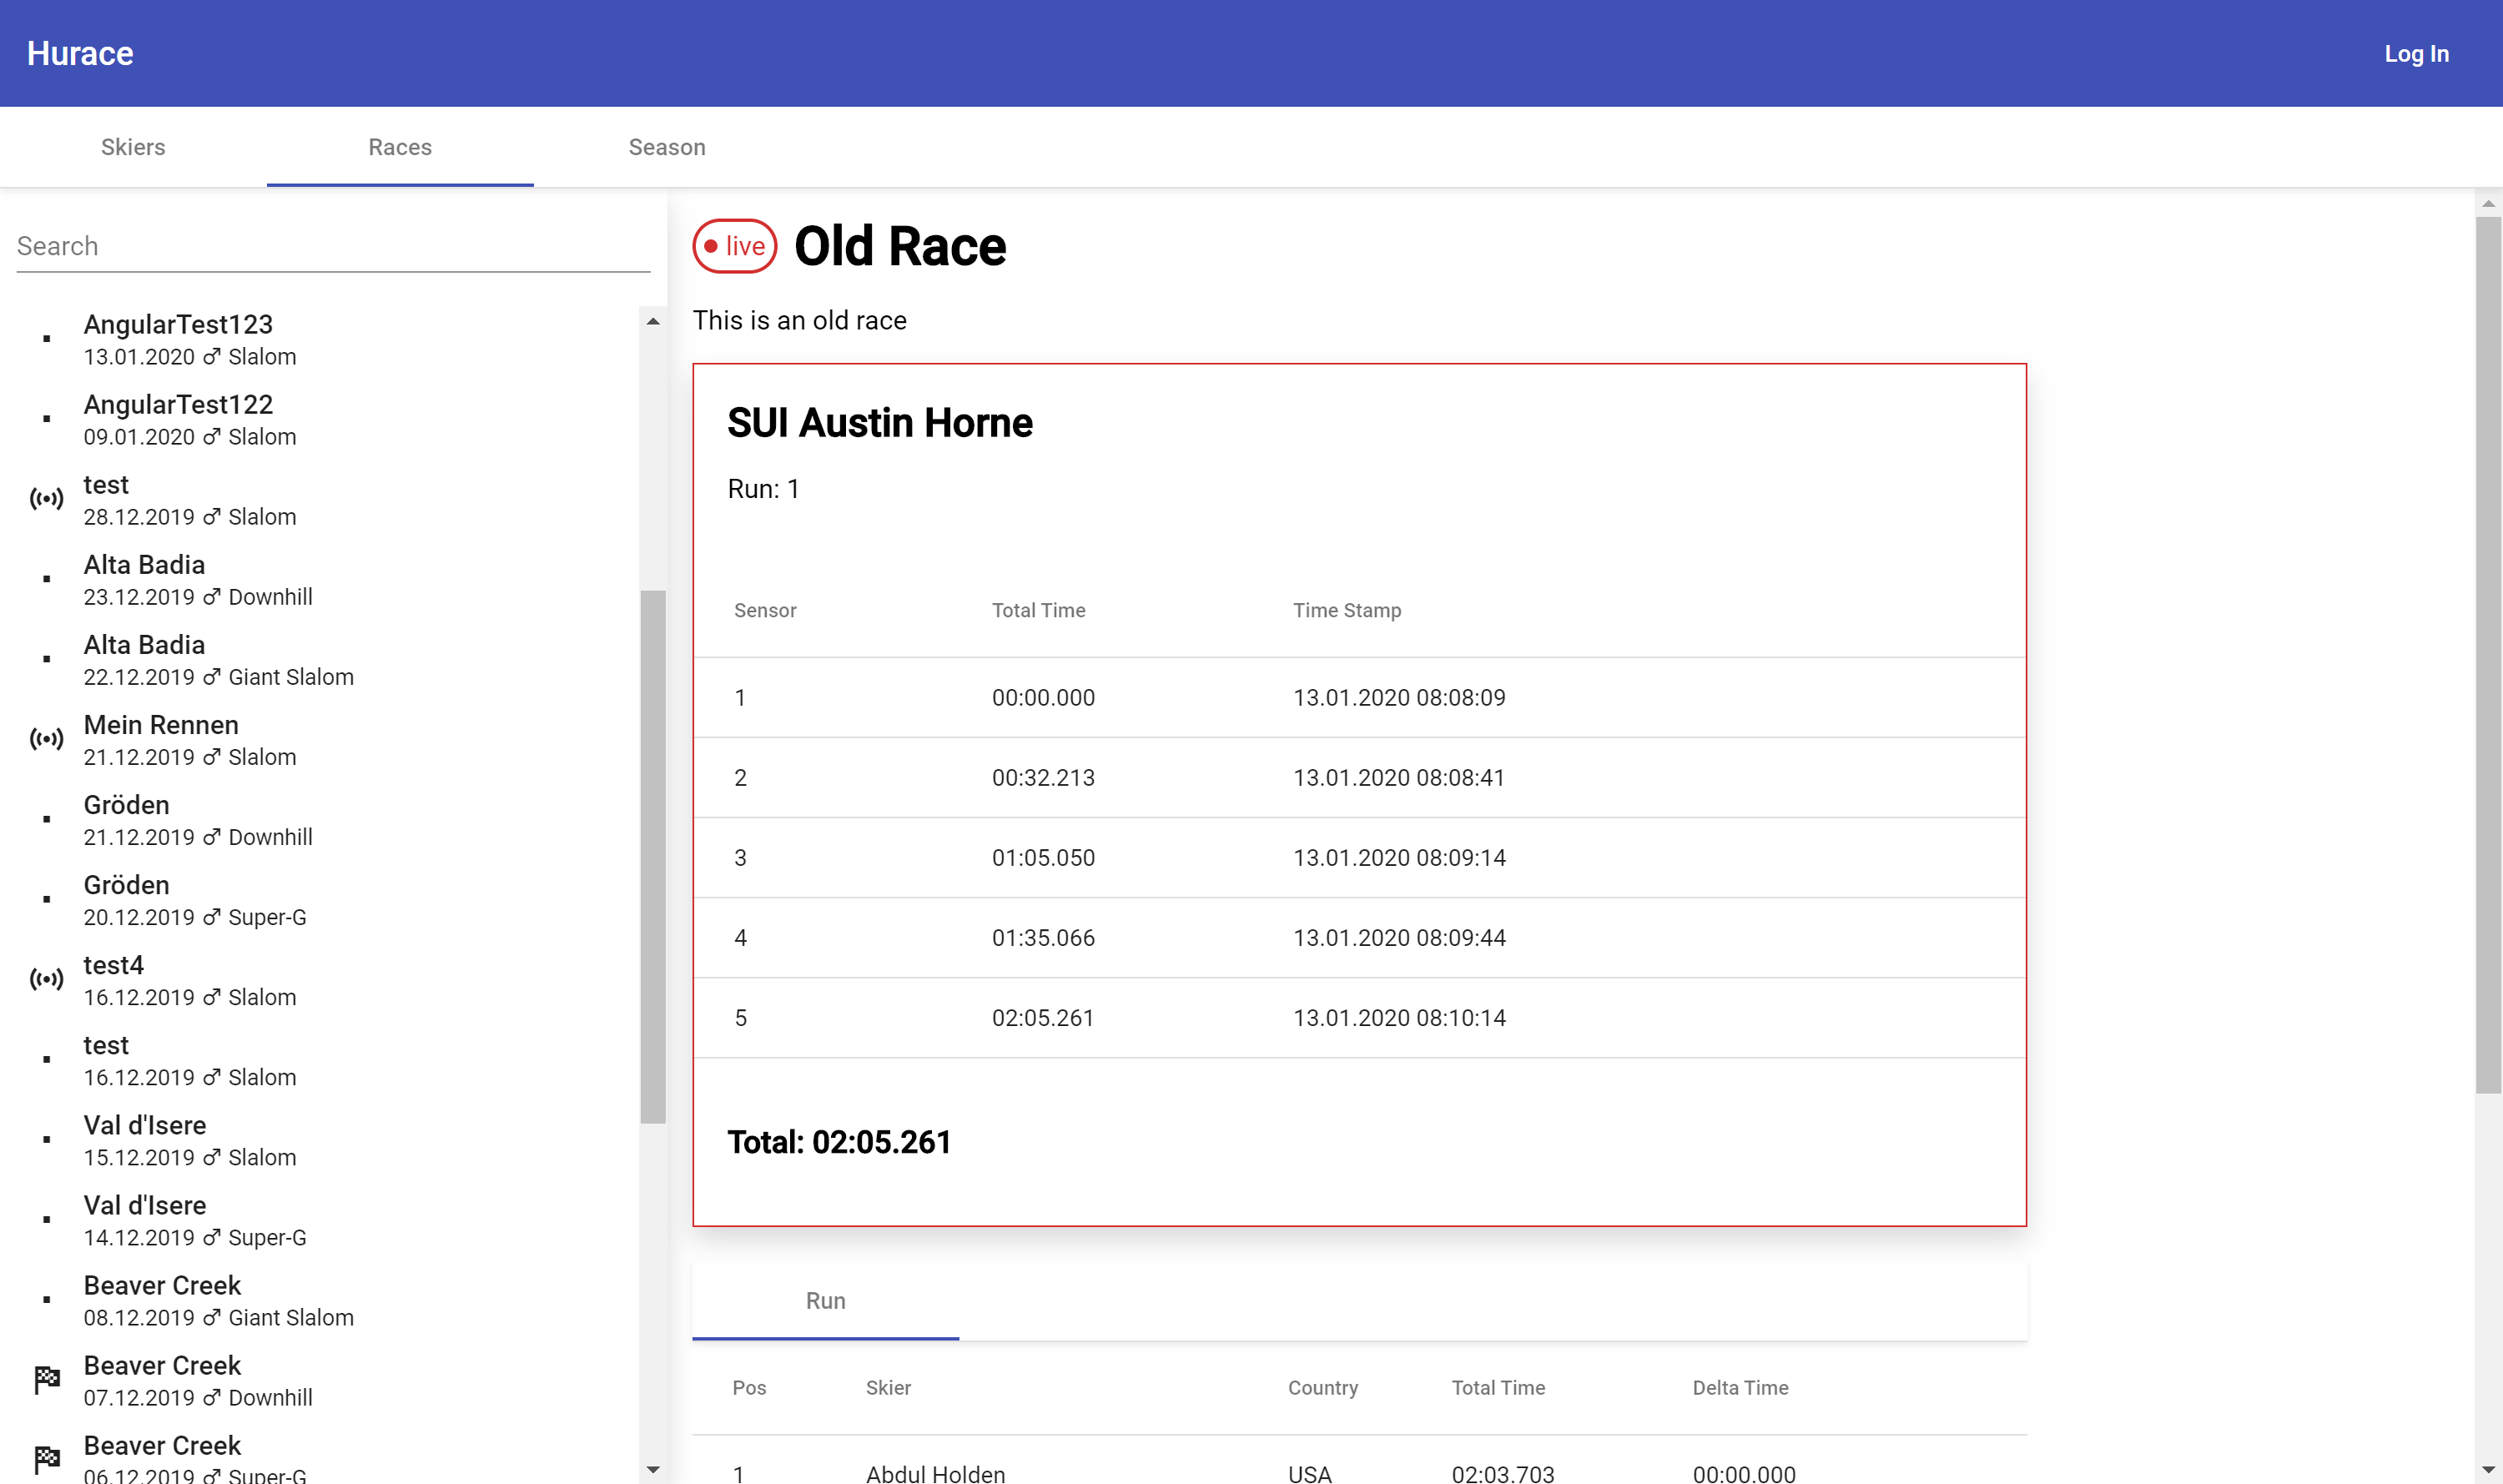
\includegraphics[width=0.9\linewidth]{images/races-live}
    \caption{Detailansicht eines laufenden Rennens}
\label{fig:races-live}
\end{figure}

\begin{figure}[H]
    \centering
    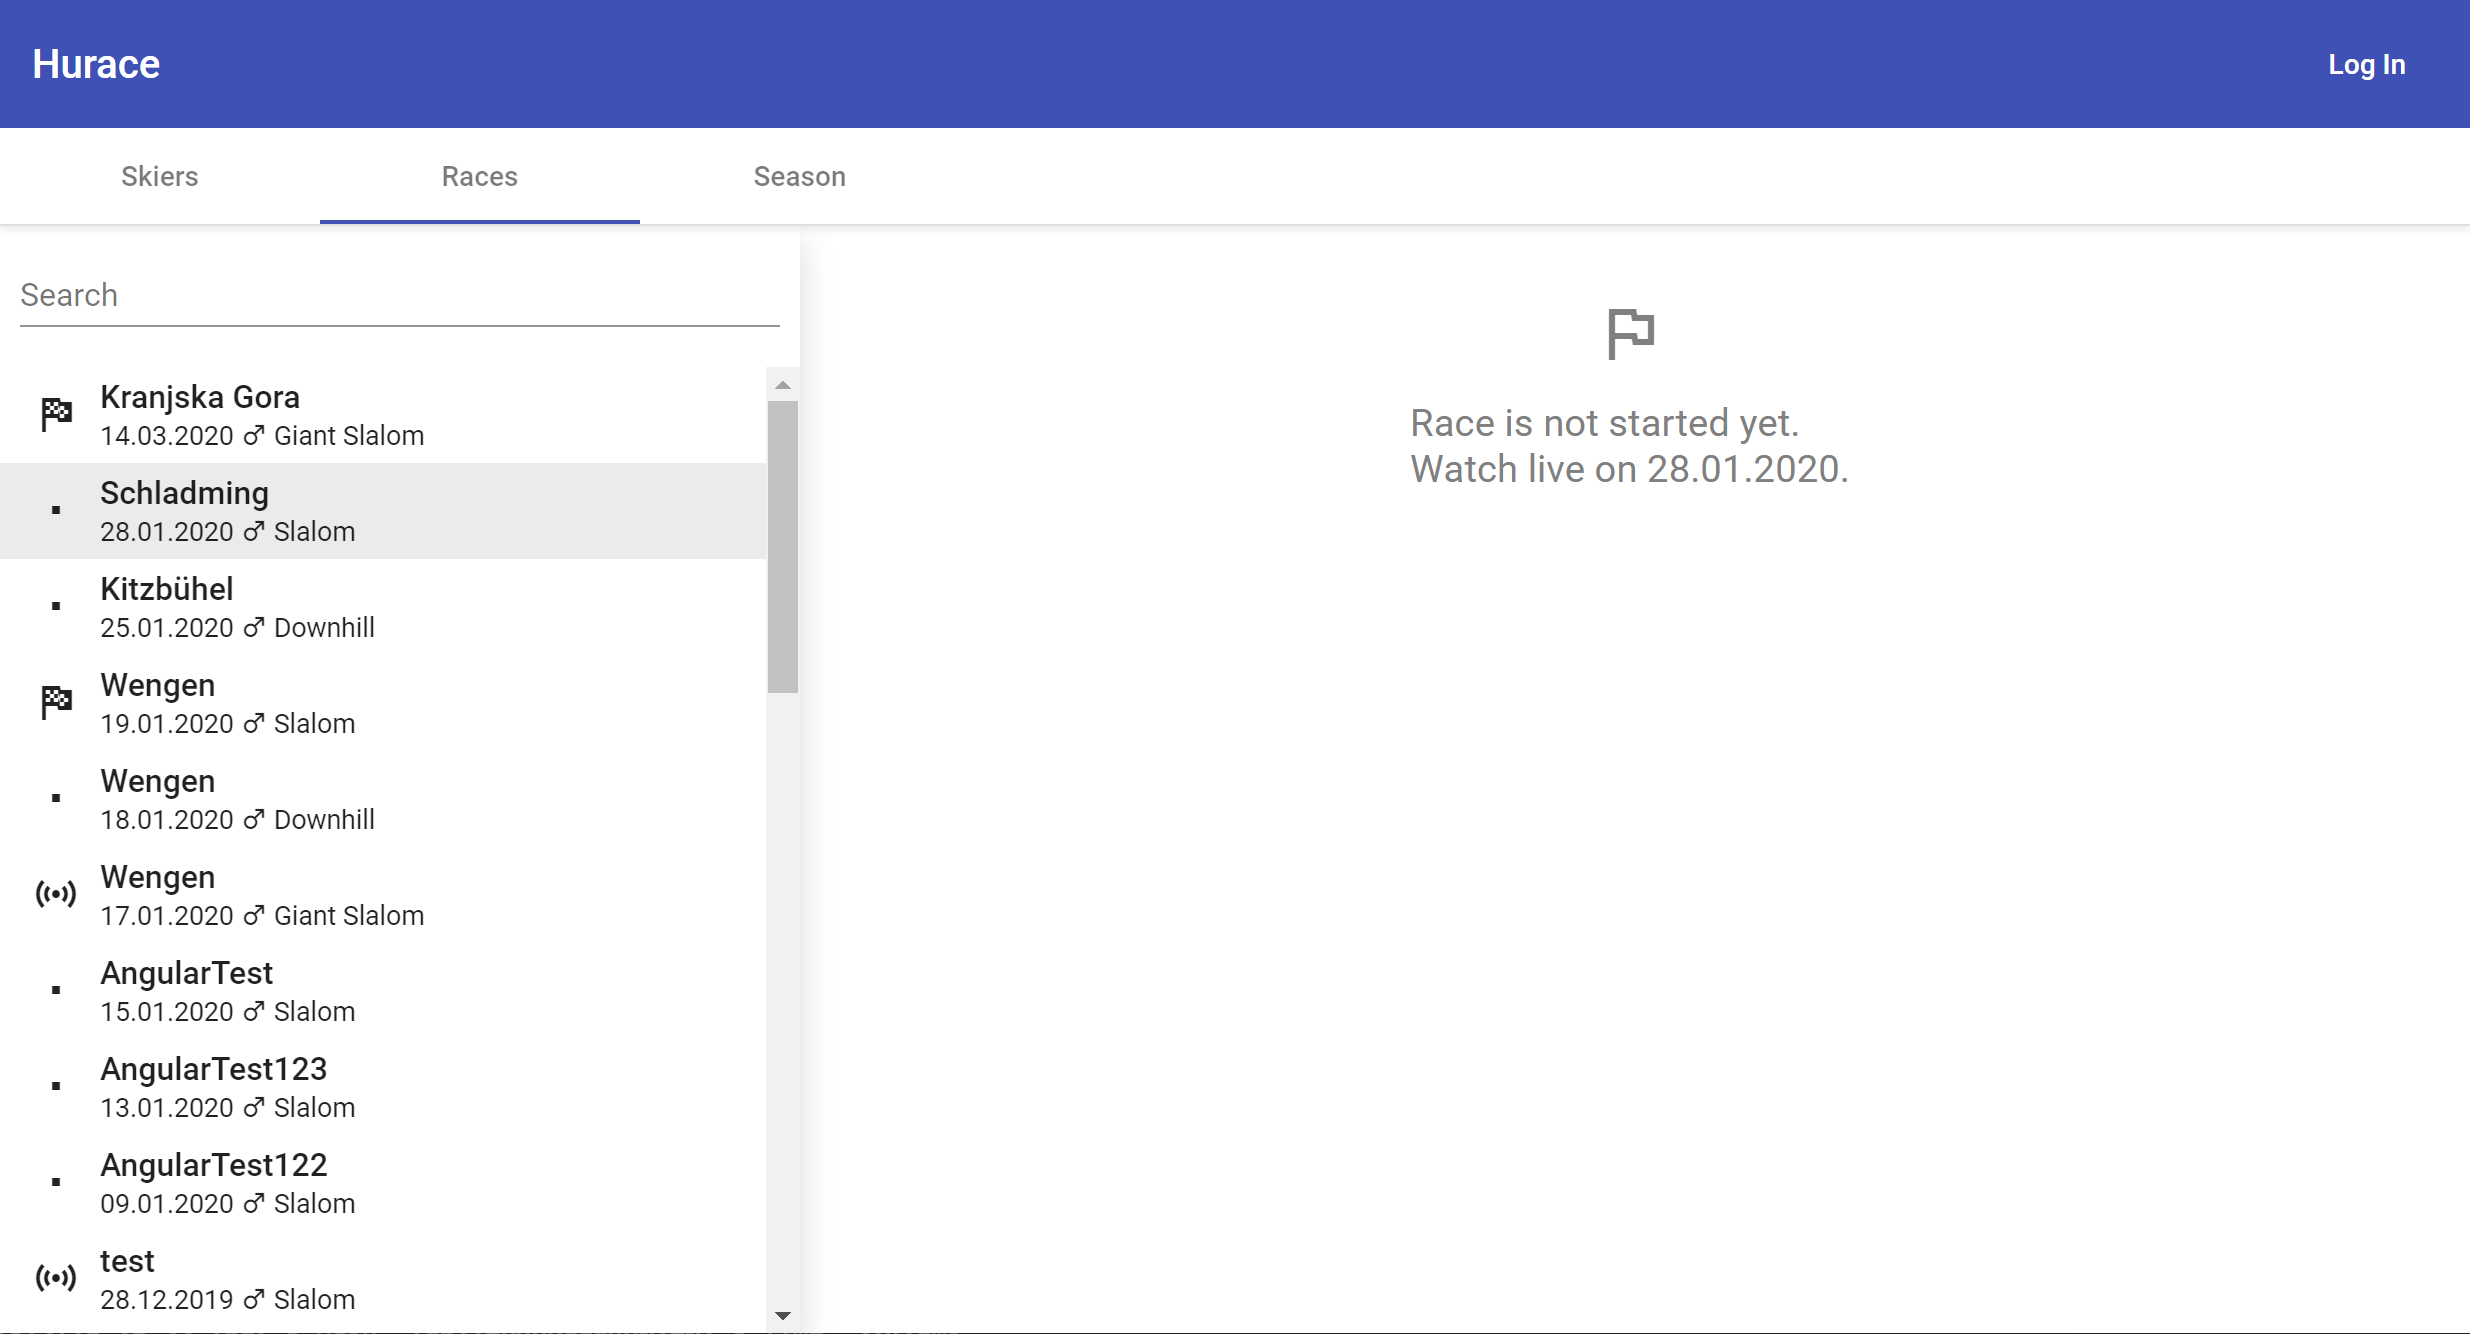
\includegraphics[width=0.9\linewidth]{images/races-not-started}
    \caption{Detailansicht eines nicht gestarteten Rennens}
\label{fig:races-not-started}
\end{figure}

\newpage
\section{Season}
Die \emph{Season}-Seite zeigt alle Rennen der aktuellen Saison nach Renntyp gegliedert an (\cref{fig:season-list}).
Mit Hilfe der Reitern (\emph{Slalom}, \emph{Giant Slalom}, \emph{Super-G} und \emph{Downhill}) kann der Renntyp gewechselt werden.
Die Liste an Rennen beinhaltet nur noch Rennen des gewählten Renntyps.
Falls ein Rennen abgeschlossen ist wird zusätzlich ein Link \emph{Show results}, der zu den Endergebnis des Rennens führt, angezeigt.
Falls ein Rennen gerade live ist wird zusätzlich ein Link \emph{Watch live}, der zu der Liveansicht des Rennens führt, angezeigt.

\begin{figure}[H]
    \centering
    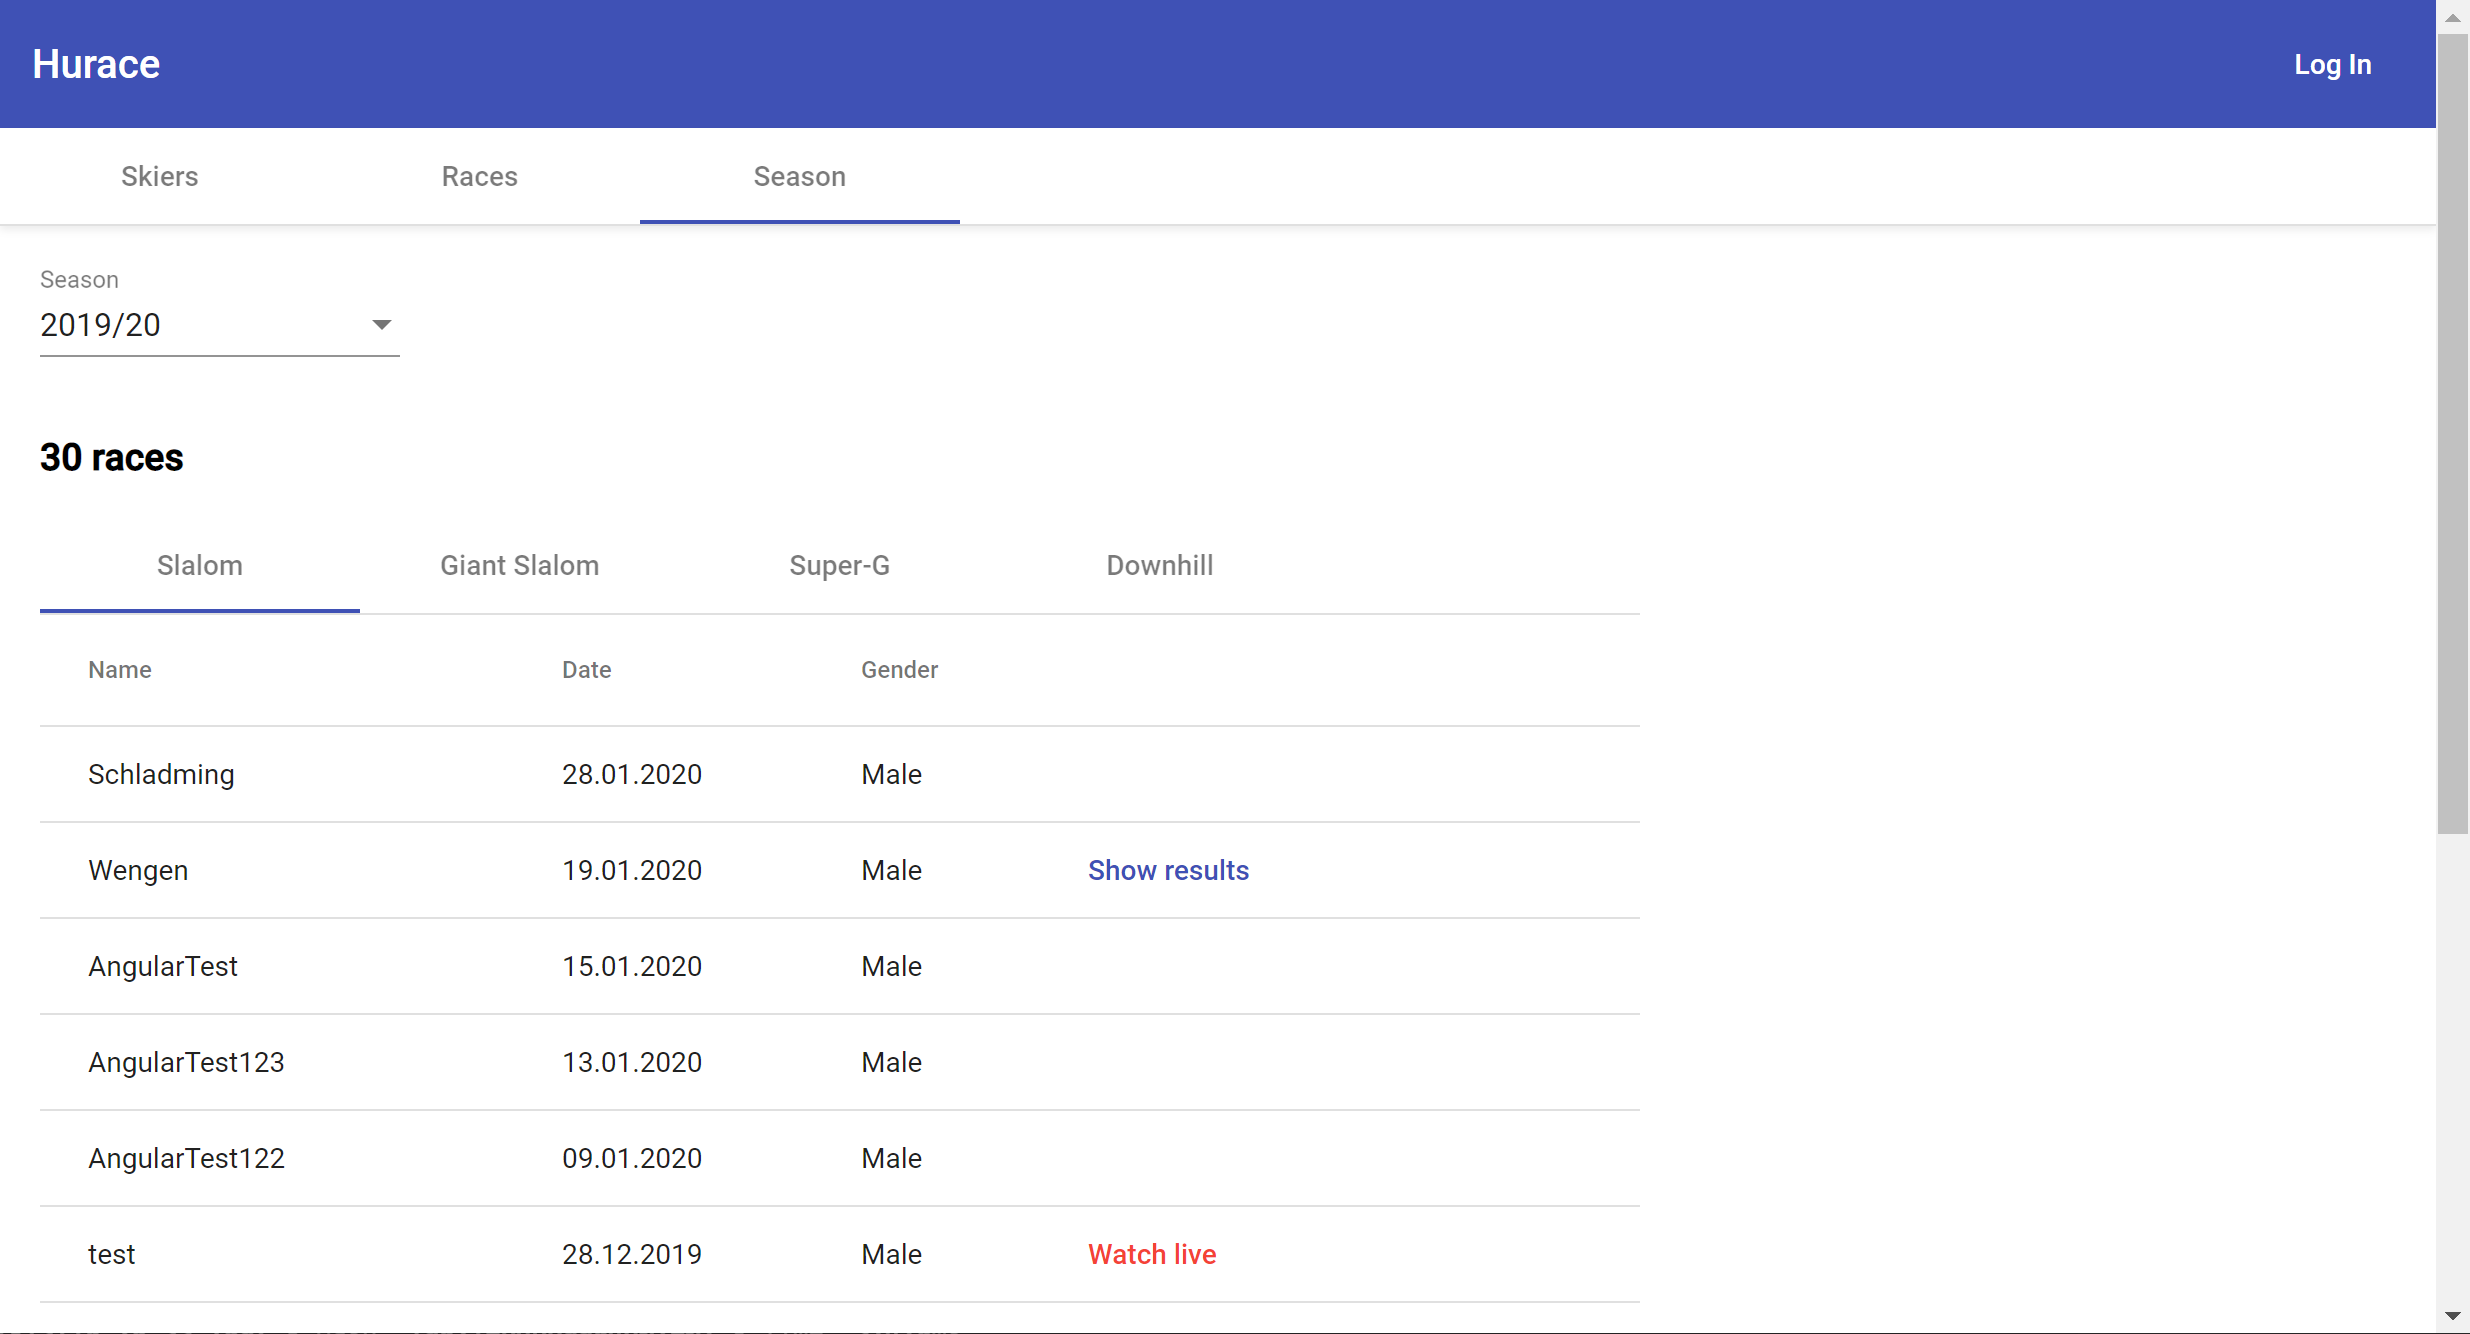
\includegraphics[width=0.9\linewidth]{images/season-list}
    \caption{Rennen nach Saison und Renntyp}
\label{fig:season-list}
\end{figure}